%Version 3 December 2023
% See section 11 of the User Manual for version history
%
%%%%%%%%%%%%%%%%%%%%%%%%%%%%%%%%%%%%%%%%%%%%%%%%%%%%%%%%%%%%%%%%%%%%%%
%%                                                                 %%
%% Please do not use \input{...} to include other tex files.       %%
%% Submit your LaTeX manuscript as one .tex document.              %%
%%                                                                 %%
%% All additional figures and files should be attached             %%
%% separately and not embedded in the \TeX\ document itself.       %%
%%                                                                 %%
%%%%%%%%%%%%%%%%%%%%%%%%%%%%%%%%%%%%%%%%%%%%%%%%%%%%%%%%%%%%%%%%%%%%%

%%\documentclass[referee,sn-basic]{sn-jnl}% referee option is meant for double line spacing

%%=======================================================%%
%% to print line numbers in the margin use lineno option %%
%%=======================================================%%

% \documentclass[lineno,sn-basic]{sn-jnl}% Basic Springer Nature Reference Style/Chemistry Reference Style

%%======================================================%%
%% to compile with pdflatex/xelatex use pdflatex option %%
%%======================================================%%

%%\documentclass[pdflatex,sn-basic]{sn-jnl}% Basic Springer Nature Reference Style/Chemistry Reference Style


%%Note: the following reference styles support Namedate and Numbered referencing. By default the style follows the most common style. To switch between the options you can add or remove “Numbered” in the optional parenthesis. 
%%The option is available for: sn-basic.bst, sn-vancouver.bst, sn-chicago.bst%  
 
%%\documentclass[pdflatex,sn-nature]{sn-jnl}% Style for submissions to Nature Portfolio journals
%%\documentclass[pdflatex,sn-basic]{sn-jnl}% Basic Springer Nature Reference Style/Chemistry Reference Style
%\documentclass[pdflatex,sn-mathphys-num]{sn-jnl}% Math and Physical Sciences Numbered Reference Style 
%\documentclass[pdflatex,sn-mathphys-ay]{sn-jnl}% Math and Physical Sciences Author Year Reference Style
%%\documentclass[pdflatex,sn-aps]{sn-jnl}% American Physical Society (APS) Reference Style
%%\documentclass[pdflatex,sn-vancouver,Numbered]{sn-jnl}% Vancouver Reference Style
%%\documentclass[pdflatex,sn-apa]{sn-jnl}% APA Reference Style 
\documentclass[pdflatex,sn-chicago]{sn-jnl}% Chicago-based Humanities Reference Style

%%%% Standard Packages
%%<additional latex packages if required can be included here>

\usepackage{graphicx}%
\usepackage{multirow}%
\usepackage{amsmath,amssymb,amsfonts}%
\usepackage{amsthm}%
\usepackage{lmodern}  % Scalable fonts for better support across sizes
\usepackage{mathrsfs}  % Since you're already using this for mathematical symbols
\usepackage[title]{appendix}%
\usepackage{xcolor}%
\usepackage{textcomp}%
\usepackage{manyfoot}%
\usepackage{booktabs}%
\usepackage{algorithm}%
\usepackage{algorithmicx}%
\usepackage{algpseudocode}%
\usepackage{listings}%
\usepackage{lmodern}  % For Latin Modern fonts (more scalable)
\usepackage{newtxmath}  % For enhanced math font support
\usepackage{hyperref}
\usepackage{lineno}
\linenumbers
\hypersetup{
    bookmarksdepth=section  % or any desired level
}
\usepackage{orcidlink}

%%%%

%%%%%=============================================================================%%%%
%%%%  Remarks: This template is provided to aid authors with the preparation
%%%%  of original research articles intended for submission to journals published 
%%%%  by Springer Nature. The guidance has been prepared in partnership with 
%%%%  production teams to conform to Springer Nature technical requirements. 
%%%%  Editorial and presentation requirements differ among journal portfolios and 
%%%%  research disciplines. You may find sections in this template are irrelevant 
%%%%  to your work and are empowered to omit any such section if allowed by the 
%%%%  journal you intend to submit to. The submission guidelines and policies 
%%%%  of the journal take precedence. A detailed User Manual is available in the 
%%%%  template package for technical guidance.
%%%%%=============================================================================%%%%

\theoremstyle{plain}
\newtheorem{theorem}{Theorem}

\theoremstyle{definition}
\newtheorem{proposition}{Proposition}

\theoremstyle{remark}
\newtheorem{example}{Example}
\newtheorem{remark}{Remark}

\theoremstyle{definition}
\newtheorem{definition}{Definition}

\raggedbottom
%%\unnumbered% uncomment this for unnumbered level heads

\begin{document}

\title[Article Title]{Lorenz Energy Cycle Climatology for the Southwestern Atlantic Cyclones}

%%=============================================================%%
%% GivenName	-> \fnm{Joergen W.}
%% Particle	-> \spfx{van der} -> surname prefix
%% FamilyName	-> \sur{Ploeg}
%% Suffix	-> \sfx{IV}
%% \author*[1,2]{\fnm{Joergen W.} \spfx{van der} \sur{Ploeg} 
%%  \sfx{IV}}\email{iauthor@gmail.com}
%%=============================================================%%

\author*[1,2]{\fnm{Danilo Couto} \sur{de Souza}}\email{danilo.oceano@gmail.com\orcidlink{0000-0003-4121-7583}}

\author[1]{\fnm{Pedro Leite da} \sur{Silva Dias}}\email{pldsdias@gmail.com\orcidlink{0000-0002-4051-2962}}

\author[3]{\fnm{Carolina Barnez} \sur{Gramcianinov}}\email{cbgramcianinov@gmail.com\orcidlink{0000-0002-3919-5226}}

\author[1]{\fnm{Ricardo} \sur{Camargo}}\email{ricamarg@usp.br\orcidlink{0000-0002-9425-5391}}

\affil*[1]{\orgdiv{Institute of Astronomy, Geophysics and Atmospheric Sciences}, \orgname{São Paulo University}, \orgaddress{\street{Rua do Matão, 266}, \city{São Paulo}, \postcode{05508-090}, \state{São Paulo}, \country{Brazil}}}

\affil[2]{\orgdiv{Climate Risk Initiative}, \orgname{IRB(re)}, \orgaddress{\street{Av. República do Chile, 330 - 4$\circ$ andar}, \city{Rio de Janeiro}, \postcode{20031-170}, \state{Rio de Janeiro}, \country{Brazil}}}

\affil[3]{\orgdiv{Institute for Coastal Systems Analysis and Modeling}, \orgname{Helmholtz-Zentrum Hereon}, \orgaddress{\street{Max-Planck-Straße, 1}, \city{Geesthacht}, \postcode{21502}, \state{Schleswig-Holstein}, \country{Germany}}}


\abstract{This study presents a climatological assessment of the Lorenz Energy Cycle (LEC) applied to South Atlantic cyclones, using a Semi-Lagrangian framework. Over 6,700 cyclones were identified from ERA5 reanalysis (1979–2020), and LEC components were computed and averaged across four objectively defined life cycle phases: incipient, intensification, mature, and decay. Results reveal a coherent energy transfer structure: baroclinic conversions dominate during intensification, while barotropic conversions peak during the mature phase and reach magnitudes 2–3 times larger than baroclinic counterparts. Diabatic generation of eddy available potential energy plays a secondary but relevant role, particularly during intensification, occasionally surpassing baroclinic contributions. Eddy kinetic energy imports are most significant during the early phases, reinforcing development. Despite substantial variability among systems, an EOF analysis shows that most cyclones share a common energy structure, with variability manifesting as amplification or suppression of specific pathways. The leading EOFs are linked to differences in cyclone intensity, genesis region, and seasonality. Among the most intense systems, distinct clusters emerge with varying energetic configurations, some dominated by baroclinic processes, others by barotropic conversions or enhanced diabatic generation. These findings demonstrate that South Atlantic cyclones encompass a spectrum of dynamical behaviors and can be classified based on their energy cycle characteristics. This study provides the first large-sample application of the Semi-Lagrangian LEC to extratropical cyclones in the South Atlantic and highlights the importance of barotropic processes in their development. The results offer a robust framework for interpreting cyclone energetics and establish a comprehensive baseline for classifying these systems.}

\keywords{Cyclone energetics, Baroclinic conversion, Barotropic conversion, Latent heat release, South Atlantic cyclones}

%%\pacs[JEL Classification]{D8, H51}

%%\pacs[MSC Classification]{35A01, 65L10, 65L12, 65L20, 65L70}

\maketitle

\section*{Acknowledgements}

The first author would like to thank the Laboratory of Applied Meteorology for Regional Meteorological Systems (MASTER) for providing the data processing infrastructure. Special thanks are extended to Jean Peres and Djalma Vieira for their invaluable technical assistance and support in the laboratory, which contributed significantly to the success of this research. CBG acknowledges the Helmholtz European Partnership “Research Capacity Building for Healthy, Productive and Resilient Seas” (SEA-ReCap, grant no. PIE-0025).

\section{Introduction}\label{sec1}

Cyclones play a crucial role in the Earth's climate system by redistributing heat, moisture, and momentum across different regions. These dynamic weather systems, contribute to the global energy balance by transferring energy from the tropics to higher latitudes. Understanding cyclone behavior is essential for improving climate projections and assessing future climate change impacts. In South America, surface cyclones influence precipitation regimes across the continent \citep{reboita2010precipitation, reboita2018extratropical, de2022hybrid} often contributing to extreme rainfall events \citep[e.g.,][]{de2021ocean,de2024extreme}, and are associated with severe meteorological hazards such as intense winds \citep{cardoso2022synoptic,de2021ocean}, high sea waves \citep{da2025classification,gramcianinov2023impact}, and storm surges along coastal areas \citep{leal2023identification,tecchiomean}. These extreme events can have profound socioeconomic impacts, including damage to coastal infrastructure, disruptions to port operations, and interruptions in oil and gas exploration. This is particularly critical in the southeastern region of South America, where large metropolitan areas, such São Paulo, Rio de Janeiro and Buenos Aires are located, as well as the Port of Santos, the largest in Latin America. 

The Lorenz Energy Cycle (LEC) is a valuable framework for understanding the conversion and flow of energy within the atmosphere, particularly in relation to synoptic and large-scale processes \citep{lorenz1967nature}. It divides the atmospheric energy budget into four main reservoirs: kinetic and available potential energy, both for zonal (mean flow) and eddy components. \citet{lorenz1955available} formulated the concept of available potential energy (APE), building upon \citet{margules1903energie} concept of energy based on the hypothetical adiabatic redistribution of atmospheric mass. The LEC serves as a foundational tool for quantifying and understanding atmospheric dynamics, by tracking energy transformations and explaining how these forms of energy are generated by adiabatic processes and dissipated by friction.

Substantial efforts have been made to estimate the LEC components for the global circulation \citep[e.g.,][]{muench1965dynamics,wiin1968intensity,hu2004variations,li2007lorenz,oort2018estimates}, to assess its projected changes under climate change scenarios \citep[e.g.,][]{hernandez2010energetics,veiga2013global,pan2017earth,michaelides2021lorenz}, and to explore its relationship with phases of the El Niño–Southern Oscillation \citep{gutierrez2009multivariate}. The LEC framework has also been applied in a range of contexts, from idealized baroclinic wave simulations \citep{kirshbaum2018sensitivity,rantanen2019sensitivity}, to rotating annulus experiments \citep{young2014lorenz}, and even to the atmospheres of other planets \citep[e.g.,][]{read2020baroclinic}. In contrast, studies examining the LEC in relation to cyclonic systems are more limited and primarily consist of case studies. These have typically focused on tropical \citep{brennan1980zonal,veiga2008analysis}, subtropical \citep{michaelides1987limited,dias2013synoptic,pezza2014large,cavicchia2018energetics}, and extratropical cyclones \citep{michaelides1992spatial,wahab2002mechanism,bulic2006limited,pezza2010environmental,dias2011energy}. Noteworthy contributions include the work of \citet{black2013universal}, which investigated explosive cyclones across all major ocean basins over a 32-year period and identified a universal signature of explosive cyclogenesis, and \citet{okajima2021cyclonic}, which quantified the contribution of migratory cyclones to global energetics, highlighting their role in accelerating westerly winds worldwide.

Although the original formulation by \citet{lorenz1967nature} was intended for global-scale studies, analyzing specific atmospheric regions is valuable for understanding the mechanisms driving the development of individual systems, such as cyclones, and the energy conversions throughout their life cycle. The initial framework for such regional analysis was introduced by \citet{muench1965dynamics}, who studied Northern Hemisphere stratospheric circulation during winter. Subsequent formulations by \citet{dutton1967theory}, \citet{vincent1973some}, and \citet{smith1980energetics} refined the approach, but it was only with \citet{brennan1980zonal} that a generalized set of equations, including both eddy and zonal components of kinetic and APE for limited regions in the troposphere, was established. However, cyclones are mobile systems that often traverse large regions \citep[e.g.]{hoskins2002new,couto2024new}. Since these studies employ the LEC within an Eulerian framework, the computational domains required to analyze cyclone energetics can become quite large \citep[e.g.]{black2013universal}, potentially incorporating other atmospheric features (e.g., migratory anticyclones, upper-level troughs, large convective systems), which limits the interpretation of results.

In this context, \citet{michaelides1999quasi} developed a Semi-Lagrangian framework for analyzing cyclone energetics, where the computational domain is movable. This approach minimizes the impact of neighboring circulations on the system's energy dynamics by employing a regional computational domain that follows the cyclone track. In the present study, we present a LEC climatology applied to cyclonic systems using such a framework, as well as the first LEC climatology (considering both Eulerian and Semi-Lagrangian frameworks) for cyclones in the Southwestern Atlantic. Over 6,700 cyclones with genesis in the Southwestern Atlantic region are analyzed, and their energy cycles are divided into distinct life cycle phases: incipient, intensification, mature, and decay. This division allows for a more comprehensive understanding of the energy flows and the dynamical mechanisms acting across each phase of the cyclone's life cycle.

\section{Materials and methods}

\subsection{Data}\label{sec:data}

For both the cyclone tracking and energetics computations, we employed the fifth-generation reanalysis from the European Centre for Medium-Range Weather Forecasts (ECMWF), known as ERA5 \citep{hersbach2020era5}. ERA5 data are produced using the Integrated Forecasting System (IFS) Cy41r2, which assimilates a wide range of observations, including satellite and in-situ measurements. It provides global coverage of numerous atmospheric, ocean-wave, and land-surface parameters at a horizontal resolution of approximately 31 km (0.25°). In this study, we utilized data from all 37 pressure levels, ranging from 1000 hPa to 1 hPa, with a temporal interval of three hours.

The cyclone tracks used in this study were obtained from the "Atlantic Extratropical Cyclone Tracks Database" \citep{gramcianinov2020data}. This database tracks the central relative vorticity of cyclones at the 850 hPa level (\(\zeta_{850}\)) using the TRACK algorithm \citep{hodges1994general, hodges1995feature} and the method outlined by \citet{hoskins2002new}. This algorithm has been employed in previous studies to assess cyclone climatologies in the South Atlantic region \citep{gramcianinov2019properties,gramcianinov2020analysis,couto2024new}. The database covers the period from 1979 to 2020 and spans the entire Atlantic Ocean within the spatial domain of 15\(^\circ\)S–55\(^\circ\)S and 75\(^\circ\)W–20\(^\circ\)E. The use of ERA5, instead of other reanalysis datasets, is justified by its higher spatial resolution, which improves cyclone detection in regions with complex orography and temperature gradients, such as the SESA region \citep{gramcianinov2020analysis}. A detailed description of the tracking methodology can be found in \citet{gramcianinov2020analysis}.

The cyclone tracking procedure employed multiple criteria to ensure accurate cyclone detection. These criteria required cyclones to have a duration of at least 24 hours and a minimum displacement of 1000 km, consistent with previous South Atlantic cyclone climatologies \citep{sinclair1995climatology,gramcianinov2019properties}. Systems that spent over 80\% of their life cycle over continental regions were excluded from the analysis to avoid counting thermal lows and lee troughs \citep[e.g.][]{crespo2021potential}. Notably, although the TRACK algorithm's calibration and sensitivity are focused on extratropical cyclones — the majority of systems in this region \citep{marrafon2022classificaccao} — the methodology does not explicitly exclude subtropical or tropical cyclones.  

To focus on the Southwestern Atlantic Ocean, only cyclones with genesis near the South American coast were considered, specifically those originating within the eastern Argentina (ARG), La Plata River basin (LA-PLATA), and southeast Brazil (SE-BR) genesis regions \citep{gramcianinov2019properties,couto2024new} (Figure~\ref{fig:combined_density_map_all_phases_regions_with_regions}). After applying these selection criteria, the database initially comprised a total of 7931 cyclones. The spatial distribution of these genesis regions and the cyclone track density for all selected systems are presented in Figure \ref{fig:combined_density_map_all_phases_regions_with_regions}. Noteworthy, in traditional cyclone studies, cyclone density is often presented for a single time step or normalized by individual tracks \citep[e.g.,][]{hoskins2005new,gramcianinov2019properties}. In contrast, Figure~\ref{fig:combined_density_map_all_phases_regions_with_regions} displays cyclone density computed across all time steps within a 5° spherical cap. Cyclones may form within the cap, move into it from adjacent regions, remain for several time steps, or pass through it entirely. Each of these time-step occurrences is counted, meaning that the density values in the figure reflect multiple temporal passages rather than unique storm events.

Among the original 7,931 cyclones, 4,445 originated in ARG (56.0\%), 1870 in LA-PLATA (23.6\%), and 1616 in SE-BR (20.4\%). However, due to data availability issues during the download process from the ERA5 database, not all cyclones could be considered in this study, resulting in a reduced total of 6,789 cyclones. These issues were related to the ERA5 API instability during the second half of 2023 and the first half of 2024, when ECMWF was migrating its data infrastructure and updating its API services. As a result, slow transfers and repeated interruptions caused incomplete or failed downloads, despite multiple attempts. This led to some cyclones being excluded from the analysis. The remaining dataset still includes a sufficiently large number of systems for robust analysis and generalization of the results. Of the 6,789 cyclones, 4,015 originated in ARG (59.1\%), 1,288 in LA-PLATA (18.9\%), and 1,486 in SE-BR (21.8\%). The reduction corresponds to a 14.4\% decrease in the number of cyclones, with region-specific reductions of 9.7\% for ARG, 31.1\% for LA-PLATA, and 8.0\% for SE-BR.


\begin{figure}[htbp]
    \centering
    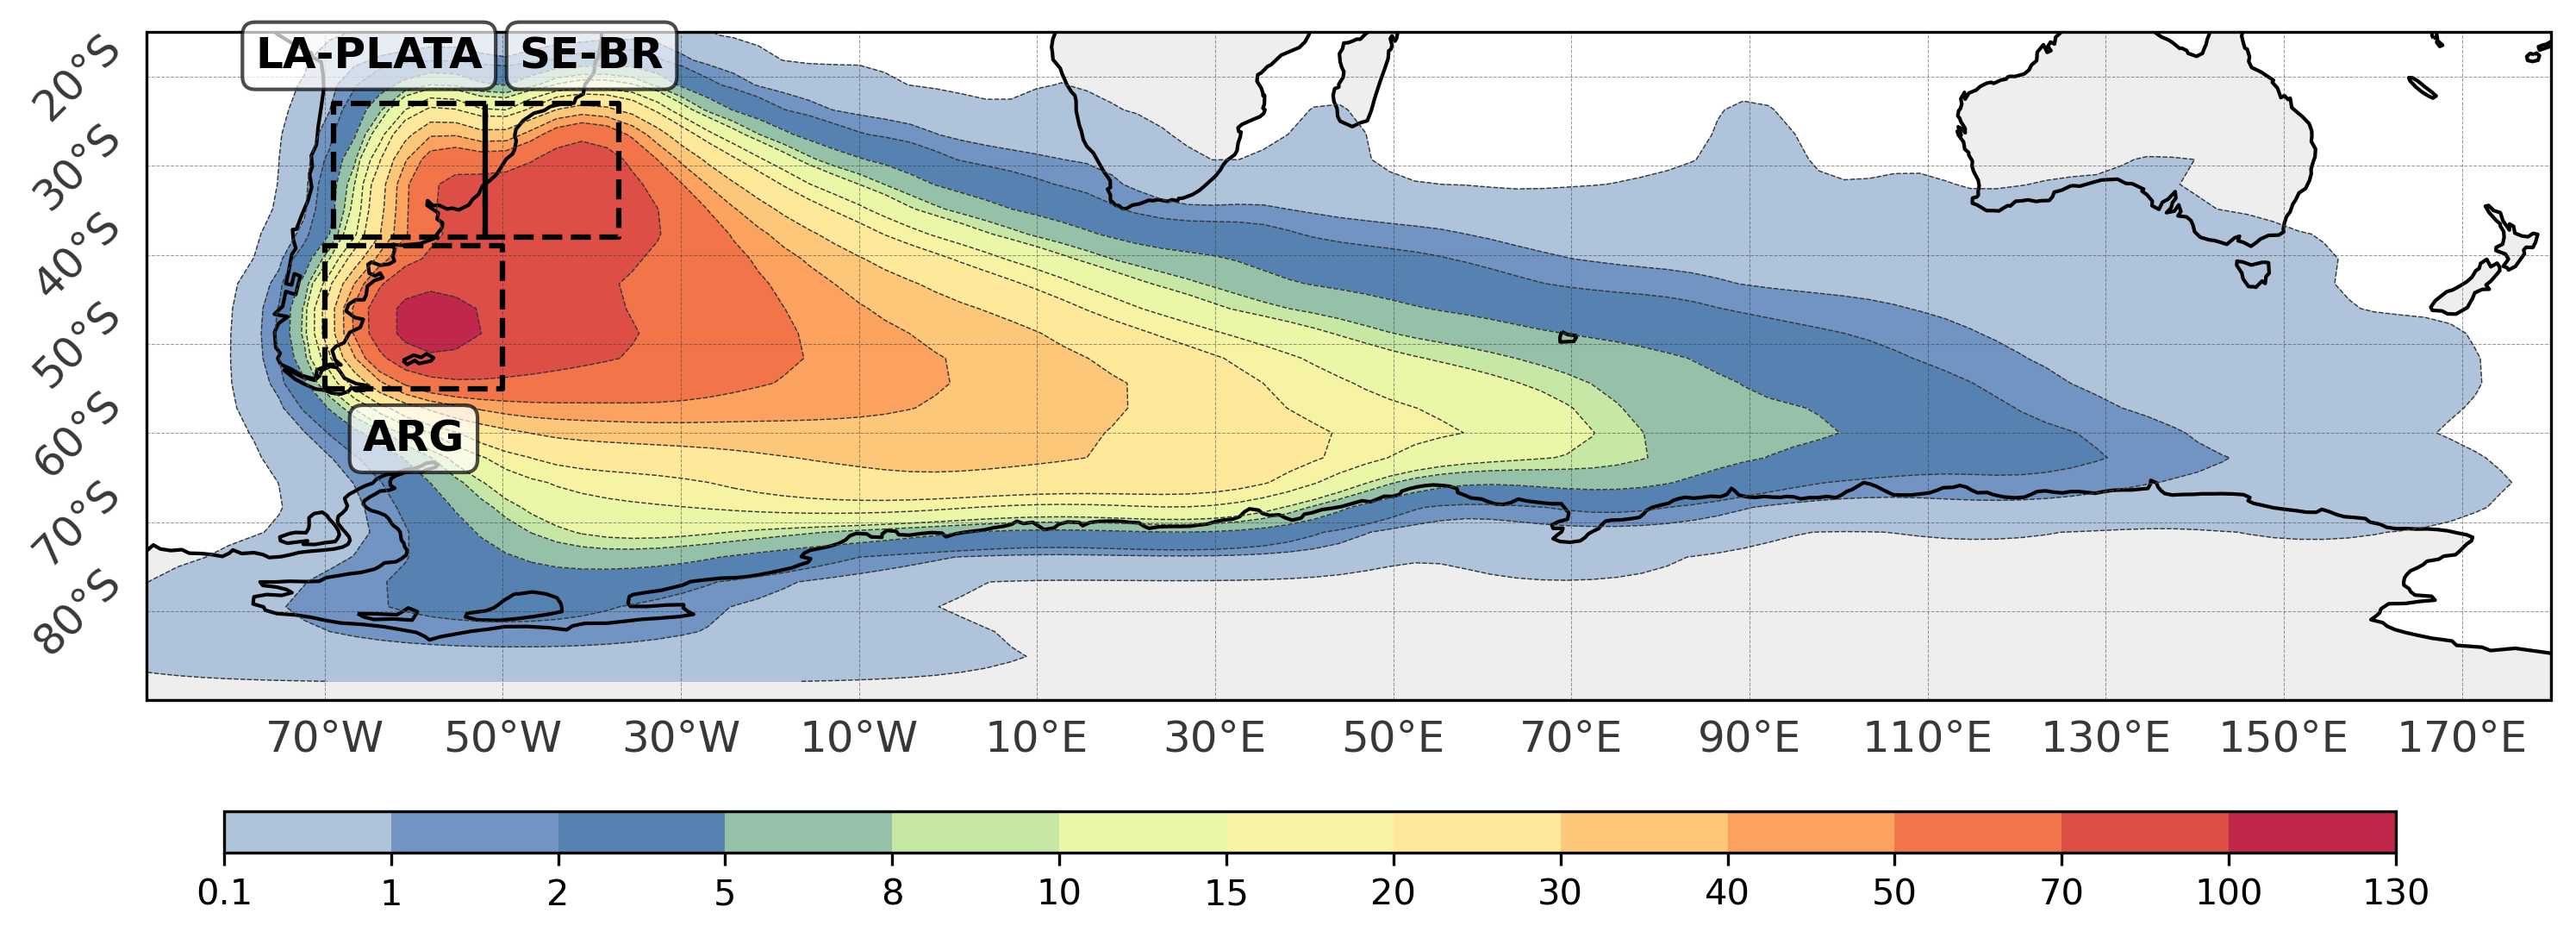
\includegraphics[width=\textwidth]{combined_density_map_all_phases_regions_with_regions.png}
    \caption{Cyclone track density for all systems analyzed in this study, highlighting the cyclogenesis regions near the South American coast (ARG, LA-PLATA, and SE-BR). The track density unit is cyclonic centers per $10^{6}$ $km^{2}$ per month.}
    \label{fig:combined_density_map_all_phases_regions_with_regions}
\end{figure}


\subsection{Lorenz Energy Cycle Computation}

For computing the LEC, we used the the open-source Python application LorenzCycleToolKit \citep{de2024lorenzcycletoolkit}. The energy budget equations for the zonal and eddy forms of APE and kinetic energy are then expressed as:

\begin{flalign}
\frac{\partial A_Z}{\partial t} &= BA_Z - C_Z - C_A + G_Z \\
\frac{\partial A_E}{\partial t} &= BA_E - C_E + C_A + G_E \\
\frac{\partial K_Z}{\partial t} &= BK_Z + C_Z - C_K + B\Phi_Z - D_Z \\
\frac{\partial K_E}{\partial t} &= BK_E + C_E + C_K + B\Phi_E - D_E 
\end{flalign}


In these equations, the atmospheric energy reservoirs are separated into zonal and eddy components of available potential energy (\(A_Z\), \(A_E\)) and kinetic energy (\(K_Z\), \(K_E\)). Energy conversions between reservoirs are represented by the following terms: \(C_A\), the conversion between zonal and eddy available potential energy (\(A_Z \leftrightarrow A_E\)); \(C_E\), the conversion from eddy available potential energy to eddy kinetic energy (\(A_E \leftrightarrow K_E\)); \(C_K\), the barotropic conversion from eddy kinetic energy to zonal kinetic energy (\(K_E \leftrightarrow K_Z\)); and \(C_Z\), the conversion from zonal available potential energy to zonal kinetic energy (\(A_Z \leftrightarrow K_Z\)). The generation of available potential energy (\(G\)) and dissipation of kinetic energy (\(D\)) are indicated by subscripts \(Z\) and \(E\), such that \(G_Z\) and \(G_E\) represent the generation of zonal and eddy available potential energy, while \(D_Z\) and \(D_E\) denote the dissipation of zonal and eddy kinetic energy, respectively. The boundary flux terms, \(BA_Z\), \(BA_E\), \(BK_Z\), and \(BK_E\), represent the import/export of available potential energy and kinetic energy across the computational domain boundaries. Additionally, the terms \(B\Phi_Z\) and \(B\Phi_E\) appear alongside \(C_Z\) and \(C_E\), respectively, as both arise from deriving the kinetic energy balances. According to \citet{muench1965dynamics}, these terms are challenging to interpret physically, but indicate processes generating kinetic energy resulting from work performed at the boundaries of the computational domain. The complete mathematical formulation of these terms can be found in the Appendix.


In these formulations, a global reference state is used to define the APE, meaning that the computed APE represents the contribution of local APE to global energetics \citep{smith1980energetics}. As a result, it does not account for regional variability, which can introduce bias in the APE computation (see \citet{novak2018local} for a thorough discussion). Despite the limitations of this methodology, the formulations by \citet{muench1965dynamics} and \citet{brennan1980zonal} still provide a valuable framework due to their simplicity, robustness, and ability to yield consistent, interpretable results, enabling direct analysis of the dynamic processes driving cyclones development \citep[][e.g.]{dias2011energy, de2025revisiting}. Moreover, while using a local APE definition \citep[][e.g.]{novak2018local} offers more precise results, it often comes with higher computational costs and does not provide the same level of direct, practical interpretability.

Following the methodologies of \citet{brennan1980zonal,michaelides1987limited,veiga2008analysis,pezza2010environmental,dias2011energy}, the program was set to compute the dissipation and generation terms as residuals, defined as:

\begin{flalign}\label{residuo_Michaelides}
RK_Z &= B\Phi_Z - D_Z + \epsilon_{KZ} \\
RK_E &= B\Phi_E - D_E + \epsilon_{KE} \\
RG_Z &= G_Z + \epsilon_{GZ} \\
RG_E &= G_E + \epsilon_{GE}
\end{flalign}

Where \(RK_Z\) and \(RK_E\) are the residual dissipation terms (zonal and eddy, respectively), \(RG_Z\) and \(RG_E\) are the residual generation terms, \(B\Phi_Z\) and \(B\Phi_E\) represent the boundary pressure work terms, and \(\epsilon\) accounts for numerical errors in the computational procedures. The set of budget equations becomes, then: 

\begin{flalign}\label{balanco_Brennan}
\frac{\partial A_Z}{\partial t} &= -C_A - C_Z + RG_Z + BA_Z \\
\frac{\partial A_E}{\partial t} &= C_A - C_E + RG_E + BA_E  \\
\frac{\partial K_Z}{\partial t} &= C_K + C_Z + BK_Z + RK_Z \\
\frac{\partial K_E}{\partial t} &= - C_K + C_E + BK_E  + RK_E 
\end{flalign}

A complete depiction of the LEC, with arrows indicating positive energy fluxes, is presented in Figure \ref{fig:LEC_chains}. This figure also highlights three primary energetic pathways (baroclinic instability, barotropic conversion, and latent heat release) which will be discussed throughout the text.

\begin{figure}[htbp]
    \centering
    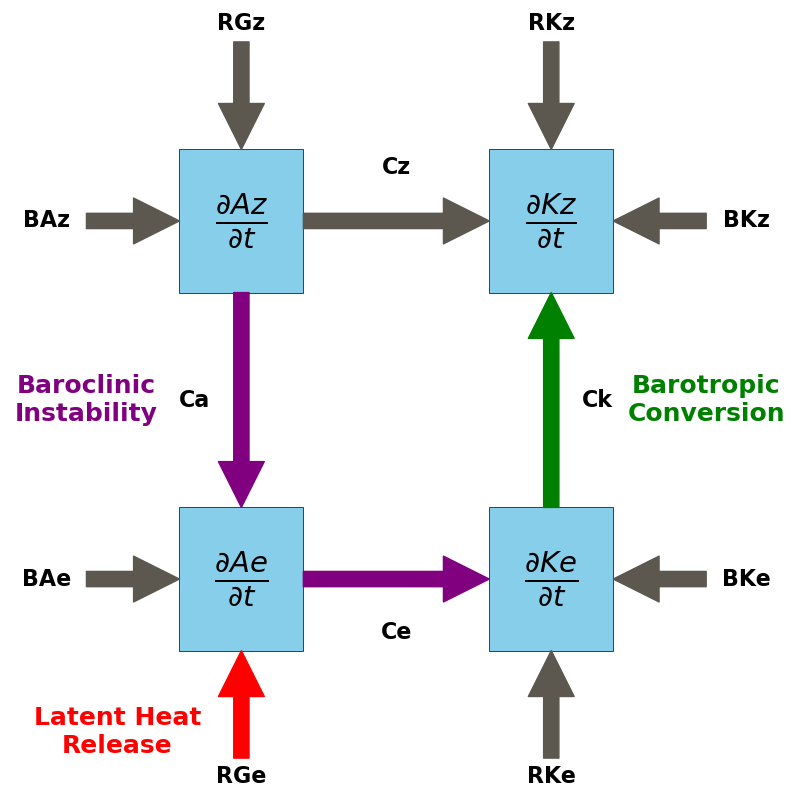
\includegraphics[width=\textwidth]{LEC_chains.png}
    \caption{Representation of the Lorenz Energy Cycle (LEC), with arrows denoting positive energy fluxes. The figure also indicates three main energetic pathways: baroclinic instability (purple), barotropic conversion (green), and latent heat release (red), which will be addressed in detail in the following sections.}
    \label{fig:LEC_chains}
\end{figure}

Here, we used a Semi-Lagrangian framework \citep{michaelides1999quasi}, aiming to minimize interactions with other non-related circulations while capturing the main structure of the cyclone. A $15^\circ \times 15^\circ$ computational domain centered at the cyclone's central position, obtained from the TRACK database, was created for each time step. Given the impracticality of manually selecting an appropriate domain size for each cyclone in the dataset, a fixed size was employed. The choice of a $15^\circ \times 15^\circ$ computational domain is justified as it is large enough to capture the effective radius of most cyclonic systems \citep{rudeva2007climatology}. The effective cyclone radius is defined as a measure of cyclone size, determined by establishing a coordinate system centered on the cyclone and measuring the distance at which the radial pressure gradient first falls to zero. This domain size also is large enough for accommodating the cyclone's synoptic structure \citep[e.g.][]{gramcianinov2019properties}.


\subsection{Analysis Methods}

A key challenge in computing the LEC for large datasets lies in the variable life durations of cyclones. Averaging energy values across an entire life cycle can obscure distinct dynamical processes tied to different stages of cyclone development, while technical limitations exist in dissecting the life cycle into distinct periods. For example, \citet{black2013universal} averaged cyclone energetics over periods of 48 hours before explosive cyclogenesis, during explosive deepening, and for 24 and 72 hours after it. However, cyclone life cycles can range from less than 24 hours to over 10 days \citep{trigo2006climatology,reboita2010south,gramcianinov2019properties}, presenting significant physical limitations to such approaches.

To address these issues, we employed Cyclophaser, an open-source Python package designed to detect cyclone life cycle phases \citep{de2025cyclophaser}. This program uses time series of relative vorticity at the system's central position and its first derivative to identify intensification, mature, and decay phases based on peaks and valleys in the vorticity and its derivative. In this study, we adopted the same life cycle detection approach as \citet{couto2024new}. After computing the LEC for each system, Cyclophaser was used to identify the life cycle phases for all analyzed cyclones, followed by the computation of mean LEC values for each phase. This approach facilitates the investigation of dynamical mechanisms specific to each development phase. For example, distinct energy fluxes are expected to dominate during the intensification and decay phases, particularly near the cyclone center. As shown by \citet{couto2024new}, approximately 60\% of the analyzed cyclones follow a classical life cycle, consisting of incipient, intensification, mature, and decay phases, while over 95\% display at least one intensification phase. A comprehensive description of the detection methodology, as well as spatial distributions and phase-specific statistics such as duration, displacement, speed, and intensity, can be found in \citet{couto2024new}.

To understand the dominant LEC variability patterns within the TRACK dataset, we performed an Empirical Orthogonal Function (EOF) analysis \citep{fukuoka1951study, lorenz1956empirical} using the Python open-source library pyEOF \citep{zheng_2021}. This analysis reduces the dimensionality of the dataset, retaining the most significant variability, and is particularly useful for uncovering underlying structures and patterns in complex environmental data. Typically, each EOF represents a spatial pattern, while the associated time series, or principal component (PC), describes the temporal evolution of that pattern. However, in this study, each EOF reflects a mode of variability derived from all LEC terms, using their average values computed separately for each cyclone life cycle phase (incipient, intensification, mature, and decay). Consequently, the PCs represent the variation across individual cyclones rather than temporal evolution, and therefore are not displayed individually, as they do not depict any meaningful temporal or spatial feature. Performing EOF analyses separately for each life cycle phase enabled a detailed investigation of the variability in cyclone energetics across distinct stages of cyclone development, as well as throughout the entire energy cycle.


To associate cyclones with predominant EOFs, we first project each cyclone's energetics onto the PCs obtained from an EOF analysis. This allows us to represent each system in terms of its contribution to the dominant modes of variability. Next, we classify cyclones into EOF(+) and EOF(-) groups, identifying systems where at least one PC reaches extreme values. Specifically, EOF(+) corresponds to cyclones where at least one PC exceeds the 90th percentile (q90), indicating a strong positive projection onto a specific mode. Meanwhile, EOF(-) are  cyclones for which at least one PC is below the 10th percentile (q10), indicating strong negative projection onto a specific mode. For each cyclone meeting these criteria, we determine its predominant EOF as the one corresponding to the PC with the highest absolute value. This ensures that each system is classified based on the mode that most strongly characterizes its structure and dynamics.

To determine the LEC patterns of the most intense systems, we first selected only the cyclones in which the maximum central vorticity at 850\,hPa exceeded the 90th percentile of the dataset. Subsequently, we applied the K-Means algorithm to the PCs of these intense cyclones to investigate whether distinct energetic characteristics could be identified among them. This clustering analysis was not performed on all cyclones, as sensitivity tests indicated that applying it to the full dataset resulted in groups that differed mainly in intensity rather than exhibiting distinct energetic behaviors (not shown); thus, intensity-based selection was necessary. 

K-Means is an unsupervised learning algorithm that partitions data into \( K \) clusters by minimizing intra-cluster variance while maximizing separation between groups based on sample similarity \citep{macqueen1967,hartiganwong1979}. The optimal number of clusters was determined using the Elbow Method, which identifies the most suitable number of clusters by plotting the within-cluster sum of squares for different values of \( K \) and locating the "elbow point," where the rate of decrease slows, indicating a balance between model complexity and performance. For this analysis, we employed the K-Means implementation from the \texttt{scikit-learn} Python package \citep{hao2019machine} and used the \texttt{yellowbrick} package for the Elbow Method \citep{bengfort2019yellowbrick}.



\section{Results}\label{sec:results}

\subsection{Climatological Features}\label{sec:climatology}

The exploratory statistical metrics for all LEC terms, presented as averages across the entire cyclone lifecycle, are shown in Table \ref{tab:lec_stats}, while their probability density functions (PDFs) are provided in Figure \ref{fig:combined_ridge}. Notably, all terms related to the zonal jets ($K_Z$, $BK_Z$, and \(\frac{\partial K_Z}{\partial t}\)) frequently exhibit statistical metrics one order of magnitude higher than their eddy counterparts within the same group ($K_E$, $BK_E$, and \(\frac{\partial K_E}{\partial t}\)), indicating significantly greater energy amount concentrated on the jet streams. Although the energy budgets were computed with the generation and dissipation terms calculated as residuals, the generation terms can be directly computed using ERA5 data. Therefore, their probability density functions (PDFs) are also shown for a more physically based analysis (Figure \ref{fig:combined_ridge}e). Furthermore, the comparison between the directly computed generation values and those estimated by residual computation provides a useful metric for evaluating the accumulation of errors in LEC computation procedure. The dissipation terms were not directly computed in the present study.


All the energy terms (\textit{Kz}, \textit{Az}, \textit{Ae}, and \textit{Ke}, Figure \ref{fig:combined_ridge}a) exhibit right-skewed distributions. Among these, $A_Z$ shows the largest variability, as reflected in its long-tail distribution, standard deviation (std), interquartile range (IQR), and range (defined as the difference between maximum and minimum values), compared to $A_E$ and $K_E$, peaking at approximately $4 \times 10^5 \, J \, m^{-2}$. Conversely, $A_E$ presents the lowest variability, peaking near $1 \times 10^5 \, J \, m^{-2}$, closer to its mean value. The kinetic energy terms, $K_Z$ and $K_E$, display similar distributions, with $K_Z$ peaking near $20 \times 10^5 \, J \, m^{-2}$ and $K_E$ peaking near $2 \times 10^5 \, J \, m^{-2}$.


\begin{table}[!htbp]
\centering
\caption[Summary Statistics of Lorenz Energetics Components]{Summary Statistics of Lorenz Energetics Components, computed as averages across the entire cyclone lifecycle: mean, median, standard deviation (std), 25th percentile (Q25), 75th percentile (Q75), interquantile range (IQR), and range. The IQR measures the range within which the central 50\% of the values fall, while the range is computed as the difference between the maximum and minimum values. The units for the energy terms ($A_Z$, $A_E$, $K_Z$, and $K_E$) are $10^5 \, J \, m^{-2}$ and $W \, m^{-2}$ for the remaining terms.}
\label{tab:lec_stats}
\begin{tabular}{lrrrrrrr}
\toprule
Term & Mean & Median & Std Dev & Q25 & Q75 & IQR & Range \\
\midrule
Az & 5.55 & 4.68 & 3.71 & 2.77 & 7.49 & 4.72 & 36.46 \\
Ae & 1.62 & 1.24 & 1.20 & 0.77 & 2.09 & 1.32 & 11.07 \\
Kz & 28.55 & 26.19 & 15.10 & 17.34 & 37.12 & 19.78 & 114.55 \\
Ke & 3.70 & 2.95 & 2.62 & 1.92 & 4.63 & 2.71 & 24.81 \\
Cz & 0.52 & 0.38 & 4.85 & -1.96 & 2.92 & 4.89 & 86.70 \\
Ca & 0.93 & 0.46 & 1.57 & 0.02 & 1.44 & 1.41 & 19.78 \\
Ck & -3.56 & -1.63 & 9.51 & -5.77 & 0.47 & 6.24 & 206.43 \\
Ce & 3.84 & 2.47 & 4.92 & 0.63 & 5.84 & 5.21 & 54.74 \\
BAz & 3.54 & 2.03 & 7.67 & -0.67 & 6.67 & 7.34 & 175.05 \\
BAe & 0.58 & 0.16 & 4.40 & -1.13 & 2.02 & 3.15 & 75.72 \\
BKz & -7.93 & -5.53 & 31.75 & -23.75 & 7.83 & 31.58 & 445.63 \\
BKe & 0.47 & 0.08 & 8.59 & -2.73 & 3.22 & 5.95 & 146.87 \\
$B\Phi Z$ & 63.87 & 49.25 & 128.05 & -9.12 & 132.35 & 141.47 & 1419.08 \\
$B\Phi E$ & 39.66 & 31.19 & 126.50 & -28.84 & 109.47 & 138.32 & 1353.99 \\
Gz & -0.31 & -0.17 & 2.66 & -1.39 & 0.81 & 2.21 & 68.74 \\
Ge & 1.17 & 0.56 & 3.14 & -0.26 & 2.21 & 2.46 & 58.39 \\
$\frac{\partial A_z}{\partial t}$ & -0.07 & -0.14 & 4.46 & -2.04 & 1.68 & 3.71 & 106.39 \\
$\frac{\partial A_e}{\partial t}$ & -0.23 & -0.10 & 1.92 & -0.85 & 0.51 & 1.35 & 48.19 \\
$\frac{\partial K_z}{\partial t}$ & 1.59 & 0.75 & 13.38 & -5.33 & 8.15 & 13.48 & 251.24 \\
$\frac{\partial K_e}{\partial t}$ & 0.28 & 0.12 & 3.18 & -1.13 & 1.58 & 2.71 & 61.50 \\
RGz & -2.17 & -1.00 & 7.60 & -5.22 & 1.56 & 6.78 & 220.06 \\
RKz & 12.56 & 8.69 & 40.49 & -8.68 & 32.71 & 41.39 & 561.24 \\
RGe & 2.10 & 1.20 & 5.15 & -0.40 & 4.21 & 4.61 & 97.25 \\
RKe & -7.59 & -4.63 & 10.62 & -11.48 & -1.04 & 10.43 & 138.42 \\
\bottomrule
\end{tabular}
\end{table}

For the conversion terms, $C_Z$, $C_K$, and $C_E$ exhibit high variability, in contrast to $C_A$. The former terms display long-tail distributions, peaking near zero, $-1$, and $2 \, W \, m^{-2}$, respectively, while $C_A$ presents a narrow distribution with a sharp peak near its mean value, close to zero (Figure \ref{fig:combined_ridge}b). The $C_Z$ probability density function (PDF), along with the mean and quantile values, and its mean value being close to the median, indicate an overall tendency for both $A_Z \rightarrow K_Z$ and $K_Z \rightarrow A_Z$ conversions. However, the positive mean and median values suggest a predominant $A_Z \rightarrow K_Z$ pathway. For $C_A$ and $C_E$, the metrics presented in Table \ref{tab:lec_stats} indicate a consistent tendency for positive conversions, corresponding to $A_Z \rightarrow A_E \rightarrow K_E$ (baroclinic chain), but with more modest $A_Z \rightarrow A_E$ conversions than $A_E \rightarrow K_E$. In the case of the $C_K$ term (barotropic conversion term), the metrics indicate a predominant negative conversion, i.e., $K_Z \rightarrow K_E$, although the positive Q75 value suggests the occurrence of events where $K_E \rightarrow K_Z$ conversions also take place.


\begin{figure}[htbp]
    \centering
    
\includegraphics[width=\textwidth]{combined_ridge.png}
    \caption{Probability density function (PDF) plots for distinct Lorenz Energetics terms, computed as averages across the entire cyclone lifecycle: (A) energy, (B) conversion, (C) boundary, (D) pressure work, (E) generation and residual, and (F) budget terms. The x-axis represents the energy values, while the y-axis represents density counts. The units for the energy terms ($A_Z$, $A_E$, $K_Z$, and $K_E$) are in $10^5 \, J \, m^{-2}$, and in $W \, m^{-2}$ for the remaining terms. Terms related to $K_Z$ are divided by 10 (*) to account for their order of magnitude difference, which would otherwise distort the visualization.}
    \label{fig:combined_ridge}
\end{figure}

For the boundary terms, $BA_E$ and $BK_Z$ exhibit similar distributions, as do $BA_Z$ and $BK_E$ (Figure \ref{fig:combined_ridge}c). The terms $BA_E$ and $BK_E$ display narrow distributions, peaking near zero, whereas $BA_Z$ and $BK_Z$ show nearly symmetrical long-tail distributions. Although for all four terms, both positive (influx) and negative (outflux) energy fluxes occur, as indicated by their negative Q25 and positive Q75 values, the peak near zero for $BA_E$ and $BK_Z$ suggests that boundary energy fluxes are typically low in most cases. In contrast, for $BA_Z$, the peak near $2 \, W \, m^{-2}$ indicates an overall tendency for energy influx, while for $BK_E$, the peak near $-2 \, W \, m^{-2}$ points to a predominant tendency for energy outflux. Meanwhile, the boundary pressure work terms ($B\Phi Z$ and $B\Phi E$) exhibit significantly higher values compared to the other boundary terms, with both presenting nearly symmetric distributions (Figure \ref{fig:combined_ridge}d). These terms show tail distributions exceeding $\pm 200 \, W \, m^{-2}$, indicating substantial variability. The physical interpretation of these terms is discussed in Section \ref{sec:comparison}.

Overall, both generation terms ($G_Z$ and $G_E$) present nearly symmetrical distributions centered near zero (Figure \ref{fig:combined_ridge}e), suggesting that in most cases, either the zonally averaged diabatic heating ($G_Z$) and the zonal deviations ($G_E$) are low, or the atmospheric stability is high. However, there are instances where this behavior is amplified ($G < 0$) or reversed ($G > 0$). In contrast, the generation residual terms ($RG_Z$ and $RG_E$) display distinct characteristics. The $RG_Z$ term is left-skewed, with a long-tail distribution and higher variability compared to $G_Z$, as indicated by its lower Q25 and higher Q75 and IQR values (Table \ref{tab:lec_stats}). Additionally, $RG_Z$ exhibits more negative mean and median values than $G_Z$, suggesting a bias toward processes such as diabatic cooling at lower latitudes and/or heat distribution mechanisms that reduce zonal temperature gradients, such as cyclonic activity. On the other hand, $RG_E$ is more symmetrical than $RG_Z$, though it still shows higher variability compared to $G_E$, as evidenced by its lower Q25 and higher Q75 and IQR values. Moreover, $RG_E$ exhibits higher mean and median values than $G_E$, indicating a bias toward overestimating the eddy effects on latent heat release and meridional temperature gradients. Therefore, the residuals suggest that the computed LEC increases the contribution of eddy motions to the atmospheric energy cycle through enhanced meridional heat transport, reducing zonal temperature gradients and enhancing convective activity within cyclone frontal structures.

Similar to the generation residual terms, each dissipation residual term displays distinct distributions (Figure \ref{fig:combined_ridge}e). The PDF for $RK_Z$ mirrors that of $RG_E$, showing modest variability. Its negative Q25 values indicate instances of net dissipation of $K_Z$. However, the high positive mean, median, Q75, and IQR values suggest that in most cases, there is a net increase of $K_Z$ related to this term, possibly due to the high $B\Phi Z$ value. In contrast, $RK_E$ shows high variability with a left-skewed, long-tail distribution. Both its Q25 and Q75 are negative, indicating that dissipation of $K_E$ frequently occurs.

\subsection{Mean Energy Values Across Life Cycle Phases}\label{sec:mean}

The use of the CycloPhaser program allowed for the application of an objective criterion to dissect the cyclones into distinct life cycle phases, enabling an investigation of their energy cycles across these phases (Figure \ref{fig:panel_lec_mean_phases}). Our analysis revealed that the mean energy flow directions rarely change across phases, although the magnitude of each term varies. However, the high standard deviation values indicate that energy fluxes frequently deviate from their mean direction.

The $A_Z$ budget term exhibits mean positive values during the incipient phase, which turn negative during the intensification and mature phases, becoming positive again during the decay phase. The mean $K_Z$ budget values are positive throughout all phases except during the mature phase. In contrast, the $A_E$ budget remains negative across the entire lifecycle, while the $K_E$ budget is positive during the incipient and intensification phases but turns negative during the mature and decay phases. However, it is important to note that the large variability observed in these terms indicates that numerous individual cases deviate significantly from these mean behaviors, including instances of opposite signs or substantially greater magnitudes.

Across the different cyclone phases, the mean behavior suggests that both baroclinic and barotropic conversions remain active, continuously providing energy to the eddies, while the adiabatic contribution from the $G_E$ term is variable throughout the lifecycle. There is a marked enhancement of baroclinic conversions from the incipient to intensification phase, which then decrease in magnitude during the mature and decay phases. Conversely, barotropic conversion peaks during the mature phase, surprisingly with a higher magnitude than the $A_E \rightarrow K_E$ conversion. The behavior of the baroclinic chain is mirrored by the $G_E$ term, which begins with negative values and, during the intensification phase, reaches a higher magnitude than the $C_A$ term. The large variability observed in these energy conversion terms indicates that multiple cyclone configurations likely exist, where either baroclinic or barotropic conversions dominate, or where both pathways coexist with varying intensities. Furthermore, the variability of the $G_E$ term suggests that, in some systems, adiabatic heating plays a significant role in cyclonic development, while in others, diabatic cooling hinders the development. The $G_Z$ term remains negative throughout the entire life cycle, with progressively decreasing values.

Throughout the life cycle, the mean values indicate imports of $A_Z$, which decrease in the mature phase but rise again during the decay phase. The mean $BA_E$ values exhibit a bimodal behavior, being positive during the incipient and intensification phases but turning negative during the mature and decay phases, though with negligible mean values in the latter. However, the large variability observed suggests that for individual cyclones, imports and exports of $A_Z$ and $A_E$ can differ substantially from these mean patterns, with some systems potentially exhibiting more pronounced or negligible boundary flux contributions.

Across all phases, the $RK_Z$ term stands out with the highest mean values, also displaying the greatest variability, as indicated by the high standard deviation values. This could be influenced by the $B\Phi Z$ term, as mentioned in the previous section. The $BK_Z$ term also presents high mean values and variability across all phases, suggesting a compensatory effect for the excess energy from the $RK_Z$ term. Lastly, the mean $RK_E$ values are negative across all phases, peaking during the mature phase, indicating significant dissipation in this phase and presenting similar values during the incipient and decay phases.


\begin{figure}[!htbp]
\centering
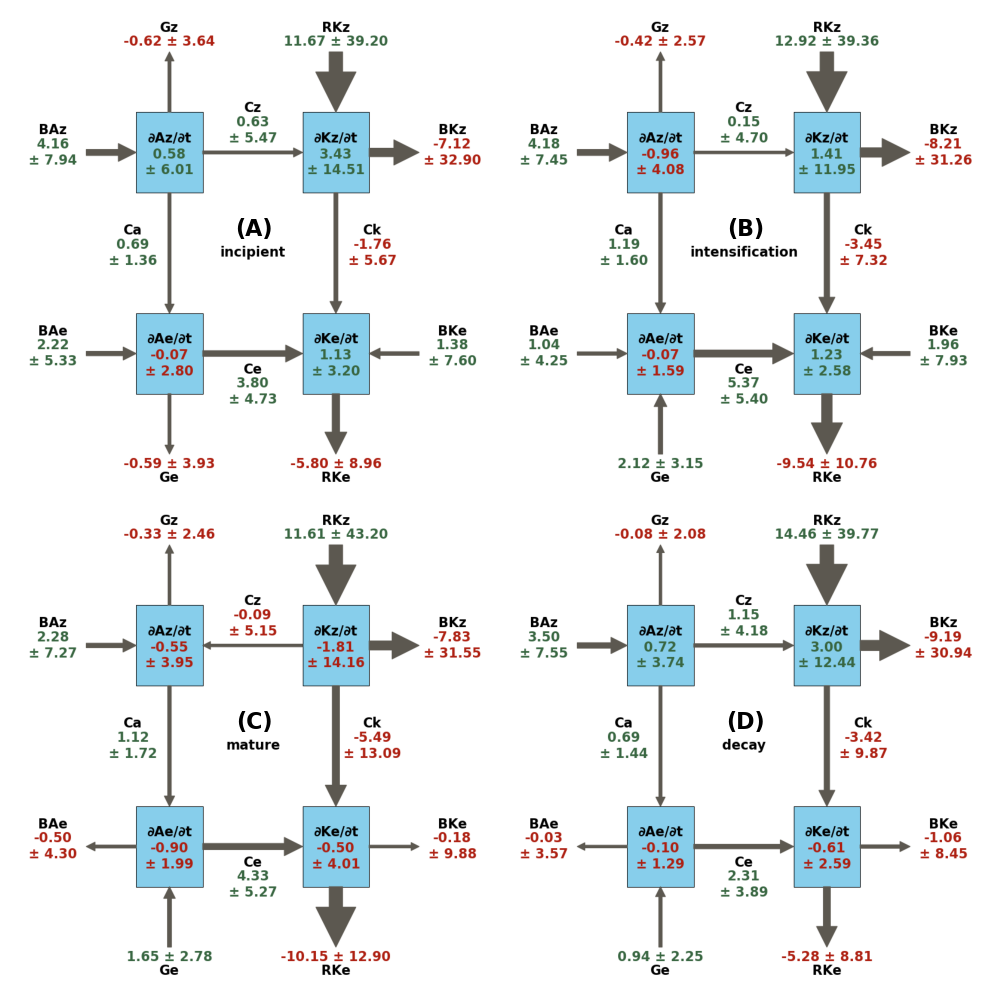
\includegraphics[width=\textwidth]{panel_LEC_mean_phases.png}
\caption{Mean values and standard deviation of the limited-area Lorenz Energy Cycle (LEC) terms for each life cycle phase : incipient (A), intensification (B), mature (C), and decay (D). Each box represents an energy component ($\, J \, m^{-2}$), with arrows showing the direction of energy flow ($\, W \, m^{-2}$). The numbers adjacent to the arrows indicate the magnitude and direction of the energy flux, with green indicating positive values and red indicating negative values}
\label{fig:panel_lec_mean_phases}
\end{figure}

\subsection{Empirical Orthogonal Function Analysis}\label{sec:eof}

To better characterize the substantial variability observed in the LEC terms, we performed an Empirical Orthogonal Function (EOF) analysis to identify distinct energetic configurations throughout the cyclone lifecycle. The first EOF accounts for 28.3\% of the total variance, followed by the second and third EOFs with 11.0\% and 10.9\%, respectively. The fourth to eighth EOFs contribute progressively less (8.2\%, 7.4\%, 5.9\%, 5.2\%, and 4.4\%), with the first four modes explaining 58.4\% of the total variance and the first eight reaching 81.3\%. These results highlight the dominant patterns of variability, with diminishing contributions beyond the initial modes. This study focuses on the first four EOFs. Although EOFs can be interpreted in terms of both positive and negative contributions, we limit our analysis to the positive phase for simplicity.

Each cyclone can be described as a linear combination of the EOFs, with the corresponding principal components (PCs) indicating how strongly each mode contributes to the system’s energetic structure. Consequently, the importance of a given EOF varies from system to system. The energy fluxes associated with each EOF represent deviations from the climatological mean (Figure \ref{fig:panel_lec_mean_phases}), either reinforcing or weakening specific energy pathways. In this way, each EOF reflects the amplification or attenuation of a characteristic energy transfer pattern within the LEC. In section \ref{sec:eof_statistics}, we examine cyclones that project strongly onto each EOF individually.

Figure \ref{fig:eof1_phases} illustrates the Lorenz Energy Cycle (LEC) terms associated with EOF 1. Across all life cycle phases, there is a consistent enhancement of moist baroclinic conversions, characterized by the positive values of the $A_Z \rightarrow A_E \rightarrow K_E$ conversions, in conjunction with an enhancement of the $G_E$ term. Furthermore, there is an increase in the $K_Z \rightarrow K_E$ conversion ($C_K$ becomes more negative), particularly during the mature and decay phases. These variations largely reinforce the mean behavior observed across the cyclone's life cycle. In addition, $A_Z$ imports are enhanced, while a negative tendency is observed in its budget and generation terms. Conversely, the $K_Z$ boundary, budget, and residual terms show a positive tendency. Lastly, the $C_Z$ term presents a weak positive signal during the incipient and decay phases, and a negative tendency during the intensification and mature phases.

\begin{figure}[!htbp]
\centering
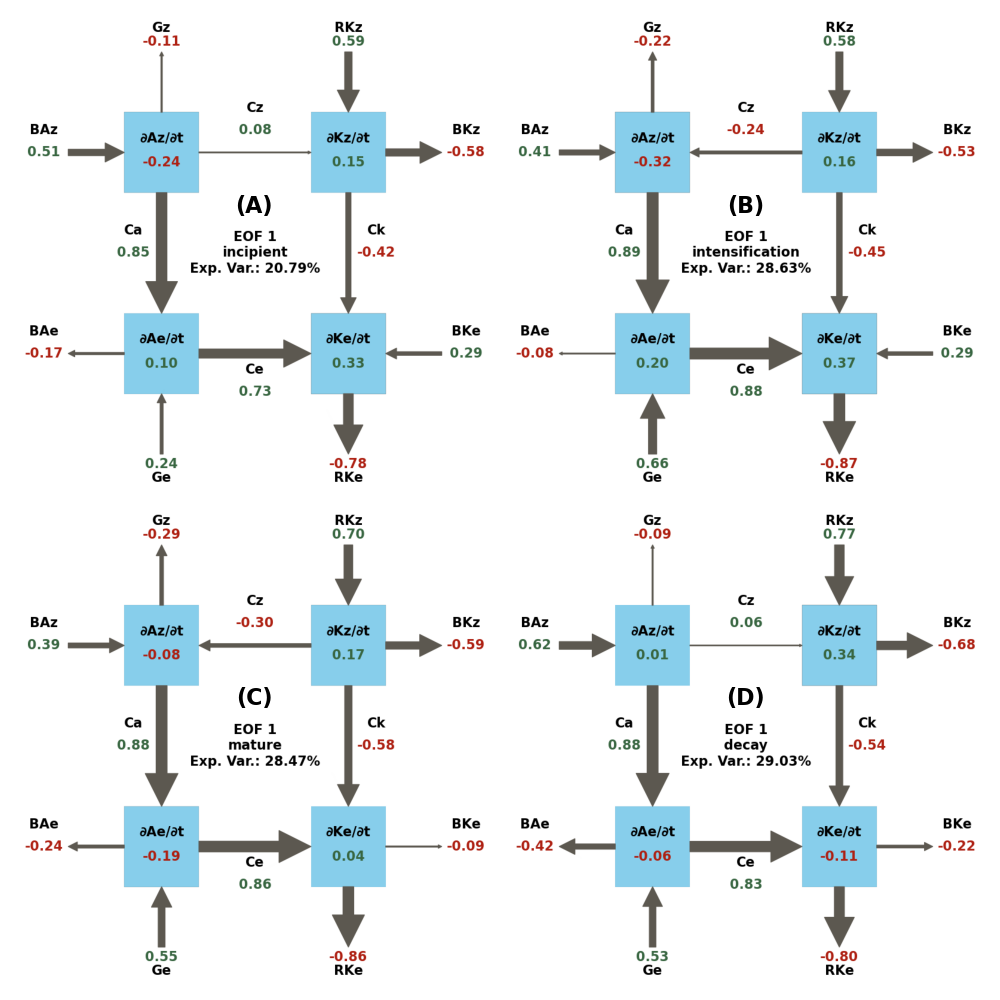
\includegraphics[width=\textwidth]{panel_LEC_EOF1.png}
\caption{Lorenz Energy Cycle (LEC) terms for the first Empirical Orthogonal Function (EOF 1) across different life cycle phases: (A) incipient, (B) intensification, (C) mature, and (D) decay.}
\label{fig:eof1_phases}
\end{figure}

During the incipient (Figure \ref{fig:eof2_phases}A) and intensification phases (Figure \ref{fig:eof2_phases}B), EOF 2 displays an overall weakening of the $C_A$ term, in contrast to EOF 1. Additionally, there is a reduction in barotropic conversions, indicating a $K_E \rightarrow K_Z$ tendency, alongside a weakening of $K_E$ imports. This reduction is compensated by an enhancement in $A_E$ imports, which appears to be the primary mechanism driving the increase in the $C_E$ term. In the mature phase (Figure \ref{fig:eof2_phases}C), the the signal for $A_E$ imports reverses in sign, and an enhancement of the moist baroclinic chain occurs, accompanied by a slight increase in $K_Z \rightarrow K_E$ conversions and a more pronounced increase in $K_E$ imports. During the decay phase (Figure \ref{fig:eof2_phases}D), both the moist baroclinic chain and $K_Z$ imports show a negative tendency. However, the enhanced barotropic conversions, coupled with a weakening of dissipation (positive tendency for $RK_E$), result in a slight yet positive tendency in $K_E$, suggesting a slower dissipation process.

\begin{figure}[!htbp]
\centering

\includegraphics[width=\textwidth]{panel_LEC_EOF2.png}
\caption{Lorenz Energy Cycle (LEC) terms for the second Empirical Orthogonal Function (EOF 2) across different life cycle phases: (A) incipient, (B) intensification, (C) mature, and (D) decay.}
\label{fig:eof2_phases}
\end{figure}

For EOF 3 (Figure \ref{fig:eof3_phases}), the role of the moist baroclinic chain diminishes in eddy development. This is evident from the weakening of the $C_E$ and $G_E$ terms across the incipient (Figure \ref{fig:eof3_phases}A), intensification (Figure \ref{fig:eof3_phases}B), and mature (Figure \ref{fig:eof3_phases}C) phases, although the $C_A$ term shows a slight enhancement during these phases. As a result, we can expect a weaker development for the incipient phase, indicated by the reduced $K_E$ budget. However, during the intensification and mature phases, the dominant source of energy shifts to barotropic conversions. During the decay phase (Figure \ref{fig:eof3_phases}D), the marginal enhancement of the $C_E$ term is driven by a slight increase in the $G_E$ term and, more importantly, by an enhancement of $A_E$ imports. Although this works in conjunction with increased $K_E$ imports, the simultaneous enhancement of $K_E \rightarrow K_Z$ conversions leads to the dissipation of eddies.


\begin{figure}[!htbp]
\centering

\includegraphics[width=\textwidth]{panel_LEC_EOF3.png}
\caption{Lorenz Energy Cycle (LEC) terms for the third Empirical Orthogonal Function (EOF 3) across different life cycle phases: (A) incipient, (B) intensification, (C) mature, and (D) decay.}
\label{fig:eof3_phases}
\end{figure}

During the incipient phase (Figure \ref{fig:eof4_phases}A) of EOF 4, the moist baroclinic chain weakens, as do the $K_E$ imports, while the barotropic conversions are enhanced. As the system progresses to the intensification phase (Figure \ref{fig:eof4_phases}B), the barotropic conversion signal becomes neutral, and the weakening of the baroclinic chain lessens, accompanied by a strengthening of $A_E$ imports. In the mature phase (Figure \ref{fig:eof4_phases}C), both the baroclinic chain and the $A_E$ and $K_E$ imports are slightly enhanced. However, the barotropic conversions reverse, signaling $K_E \rightarrow K_Z$ conversions, indicating a transfer of energy from eddy kinetic energy to zonal kinetic energy. In the decay phase (Figure \ref{fig:eof4_phases}D), the signal of baroclinic conversions returns to its initial weakened state and $A_E$ imports are reduced, while $K_E$ are enhanced. Although the $K_E \rightarrow K_Z$ conversions are enhanced, they are counterbalanced by the $K_E$ imports, leading to a slower eddy dissipation (higher tendency for $K_E$ the budget).

\begin{figure}[!htbp]
\centering

\includegraphics[width=\textwidth]{panel_LEC_EOF4.png}
\caption{Lorenz Energy Cycle (LEC) terms for the fourth Empirical Orthogonal Function (EOF 4) across different life cycle phases: (A) incipient, (B) intensification, (C) mature, and (D) decay.}
\label{fig:eof4_phases}
\end{figure}

Here we present a summary of the energy pathways that were enhanced for each EOF, indicating the increased contribution to cyclone development (i.e., $K_E$ increases). During EOF1, both the moist baroclinic and barotropic chains are enhanced, with increased imports of $K_E$ during the incipient and intensification phases. For EOF2, cyclone development is characterized by the enhancement of the $BA_E \rightarrow A_E \rightarrow K_E$ chain during the incipient and intensification phases, followed by an increase in $K_E$ imports during the mature phase. For EOF3, during the incipient phase, there is an enhancement of $K_E$ imports, which is followed by an increase in barotropic conversions during the intensification and mature phases. For EOF4, barotropic conversions are enhanced during the incipient phase, with nearly neutral baroclinic and barotropic conversions during intensification, and an enhanced baroclinic chain along with $K_E$ imports during the mature phase. During cyclone decay, EOF1 shows an enhancement in dissipation, EOF2 and EOF4 present an enhancement in exports of $K_E$, and EOF3 exhibits an increase in $K_E \rightarrow K_Z$ conversions.

\subsection{Characteristics of Cyclones Based on EOF Signal}\label{sec:eof_statistics}

In this section, as the characteristics of the systems associated with each EOF are analyzed, the EOF signal becomes relevant, necessitating a distinction between systems related to positive EOF signals — EOF(+) — and negative EOF signals — EOF(-), respectively. EOF1 accounts for the largest number of cyclones among the first four EOFs for both EOF(+) and EOF(-). For EOF(+), it is followed by EOF2, EOF3, and EOF4, while for EOF(-), it is followed by EOF3, EOF2, and EOF4, respectively (Figure \ref{fig:panel_2x2_metrics_q90_vs_q10}a). The track densities for the cyclones associated with EOF(+) are presented in Figure \ref{fig:density_panel_q90}, while those for EOF(-) are shown in Figure \ref{fig:density_panel_q10}. For EOF1(+), the track density maximum extends from SE-BR and LA-PLATA toward the ARG region, highlighting the significant contribution of systems originating in the former regions compared to the latter, as also indicated in Figure \ref{fig:panel_2x2_eof_statistics}a. In contrast, for the remaining EOFs(+), the track density maximum is located near the ARG region, as most systems originate there. An exception is observed in EOF3(+), where the track density maximum extends northeastward due to the increased contribution of SE-BR systems to this EOF.


\begin{figure}[!htbp]
\centering
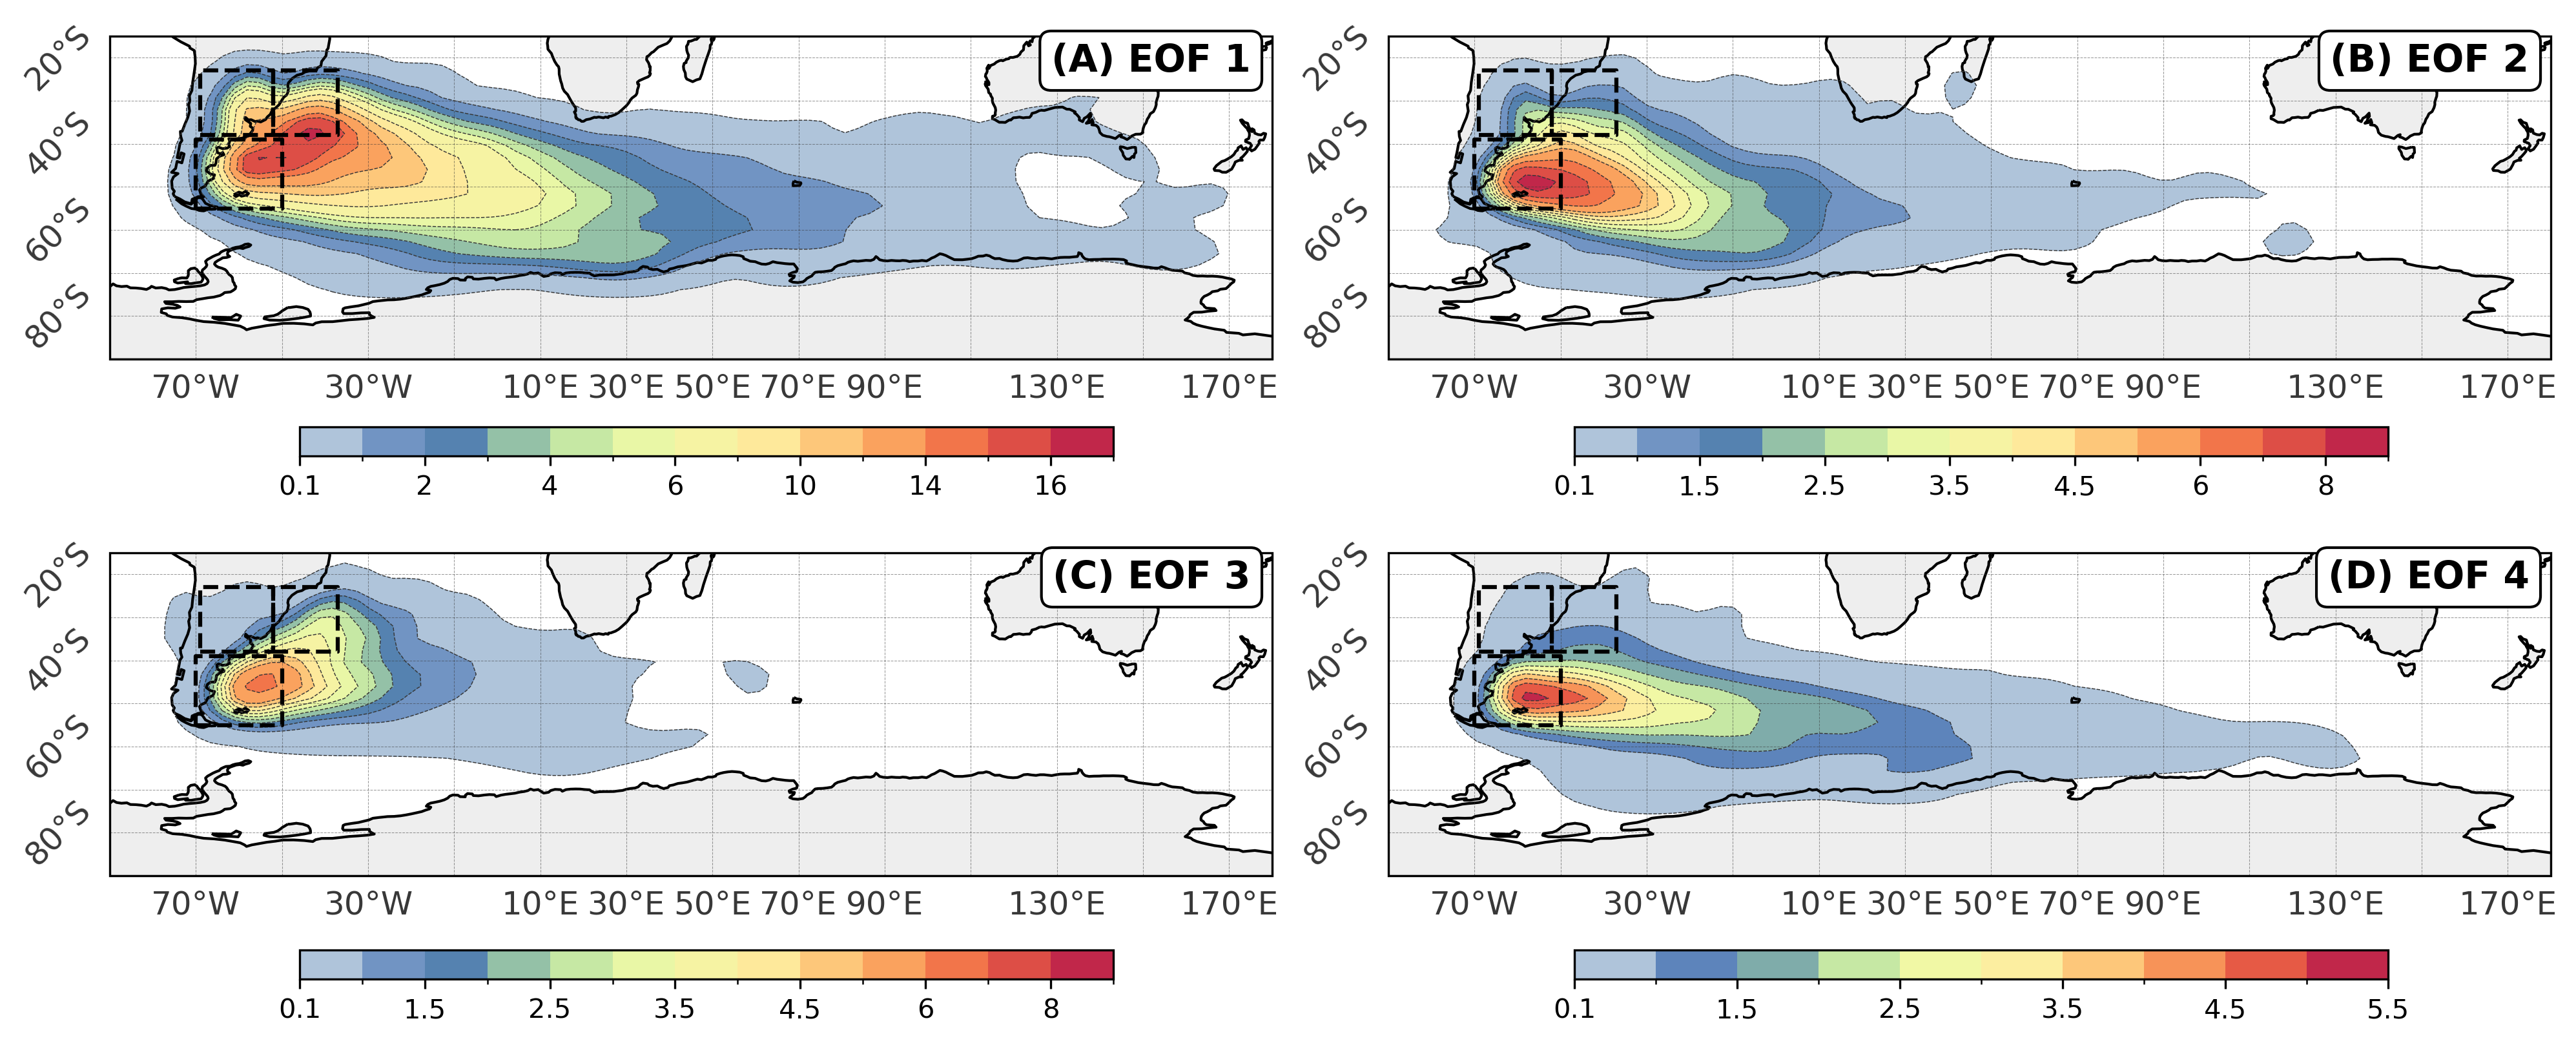
\includegraphics[width=\textwidth]{density_panel_q90.png}
\caption{Cyclone track density for the systems associated with EOFs(+): (A) EOF1, (B) EOF2, (C) EOF3, and (D) EOF4. The track density unit is cyclones per $10^{6}$ km$^{2}$ per month. The dashed rectangles mark the genesis regions shown in Figure \ref{fig:combined_density_map_all_phases_regions_with_regions}.}
\label{fig:density_panel_q90}
\end{figure}

\begin{figure}[!htbp]
\centering
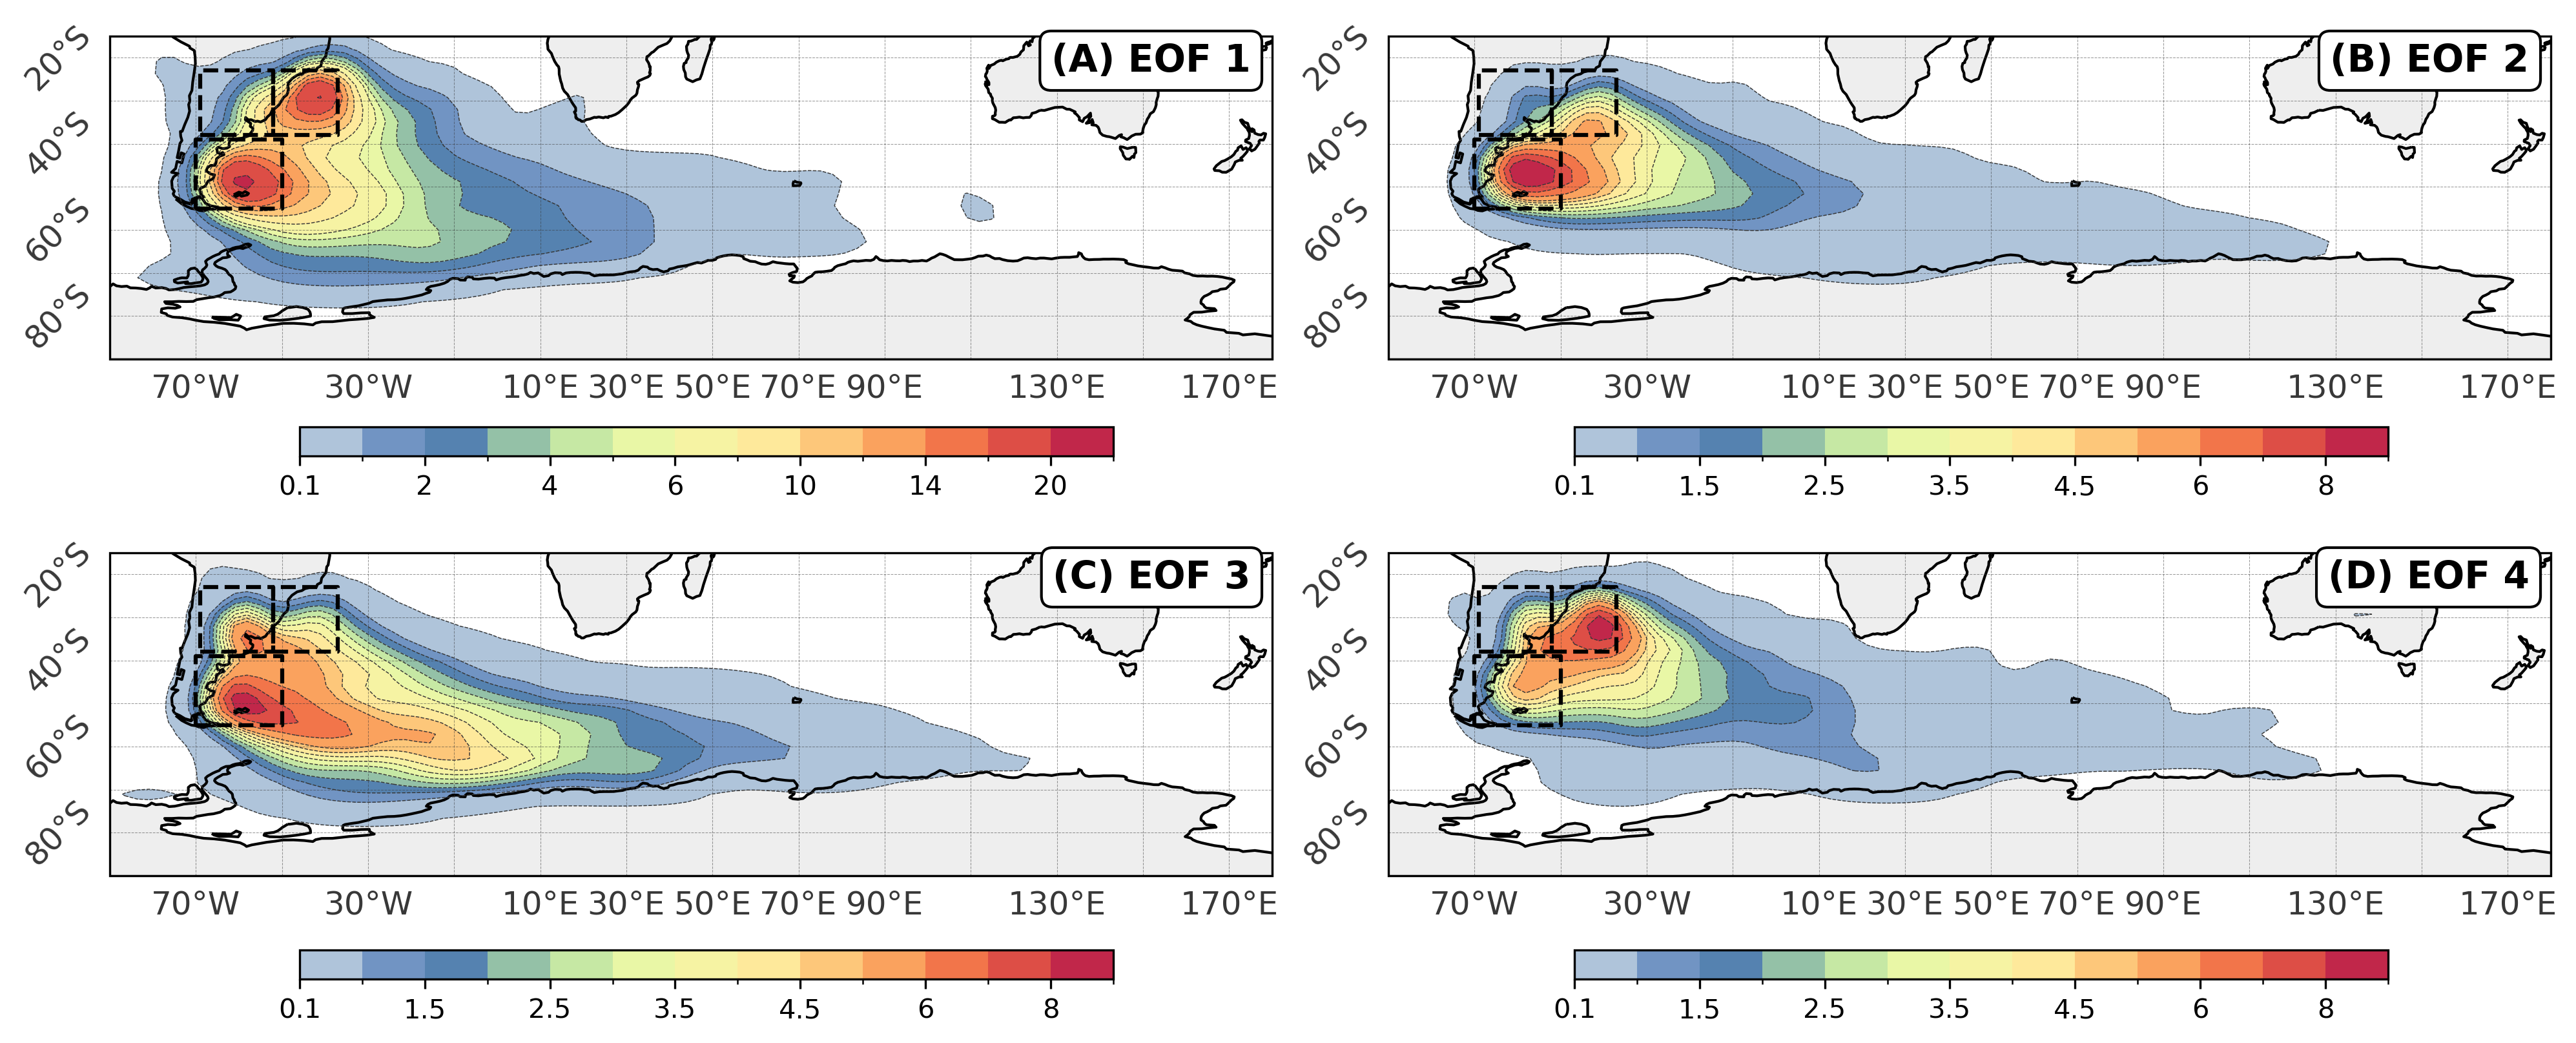
\includegraphics[width=\textwidth]{density_panel_q10.png}
\caption{Cyclone track density for the systems associated to EOFs(-): (A) EOF1, (B) EOF2, (C) EOF3 and (D) EOF4. The track density unit is cyclonic centers per $10^{6}$ $km^{2}$ per month. The track density unit is cyclones per $10^{6}$ km$^{2}$ per month. The dashed rectangles mark the genesis regions shown in Figure \ref{fig:combined_density_map_all_phases_regions_with_regions}.}
\label{fig:density_panel_q10}
\end{figure}

Meanwhile, EOFs(-) exhibit a more variable behavior. EOF1(-) displays two track density maxima: one near SE-BR and another near ARG, as fewer systems originate from LA-PLATA for this EOF (Figure \ref{fig:panel_2x2_eof_statistics}c). EOF2(-) is predominantly influenced by ARG systems, whereas EOF3(-) shows an increased contribution from LA-PLATA systems, with a primary track density maximum near ARG and a secondary maximum over the La Plata River mouth. Lastly, EOF4(-) presents a track density maximum between LA-PLATA and SE-BR, reflecting the increased relative contribution of systems from these regions to this EOF.

Despite regional differences in track density maxima, nearly all EOFs exhibit a common pattern of cyclone tracks extending southeastward across the South Atlantic (Figures~\ref{fig:density_panel_q90} and \ref{fig:density_panel_q10}), with the exception of EOF3(+).  Some systems display exceptional mobility, reaching as far as $150^{\circ}$E. This behavior aligns with the typical lifecycle of cyclonic systems originating near the South American coast, where cyclones generally develop near the coastal region, mature as they propagate southeastward, and decay closer to the Antarctic region \citep{couto2024new}.

As shown in Figure \ref{fig:panel_2x2_eof_statistics}b, EOF1(+) and EOF4(+) systems predominantly originate during JJA, while EOF2(+) and EOF3(+) genesis events are more evenly distributed across the seasons. For EOFs(-), EOF1(-) systems occur mainly during DJF, whereas EOF4(-) systems are more frequent during DJF and MAM. In contrast, EOF2(-) and EOF3(-) systems are predominantly observed during JJA and SON (Figure~\ref{fig:panel_2x2_eof_statistics}d). The seasonal distribution of EOF2(+) and EOF3(+) systems aligns with the expected behavior, as ARG systems are well-distributed throughout the year \citep{gramcianinov2019properties,crespo2021potential}. However, for the remaining EOFs, the observed behavior suggests that seasonal variations are linked to changes in the systems' energetics.

\begin{figure}[!htbp]
\centering

\includegraphics[width=\textwidth]{panel_2x2_q90_vs_q10.png}
\caption{Genesis proportion and seasonal occurrences of EOFs. (A) Genesis proportion for EOF(+), (B) Seasonal occurrences for EOF(+), (C) Genesis proportion for EOF(-), and (D) Seasonal occurrences for EOF(-). The colors represent different genesis regions (ARG, LA-PLATA, SE-BR) in (A) and (C), while in (B) and (D), the colors correspond to seasonal distributions (DJF, MAM, JJA, SON).}
\label{fig:panel_2x2_eof_statistics}
\end{figure}

\subsection{Groups of Intense Systems}

While the previous sections examined the LEC for all cyclonic systems in the South Atlantic — analyzing both the mean behavior and its associated variability through EOF analysis — this section focuses on the energetic groups associated with the most intense cyclones in the dataset. The K-Means algorithm was applied to the first eight PCs of the selected cyclones, identifying five distinct LEC groups, as determined by the Elbow Method. Following the cluster identification analysis, the energetic characteristics of the systems were reconstructed, with the mean behavior for each group represented in Figure \ref{fig:LEC_clusters_std}.

\begin{figure}[!htbp]
\centering
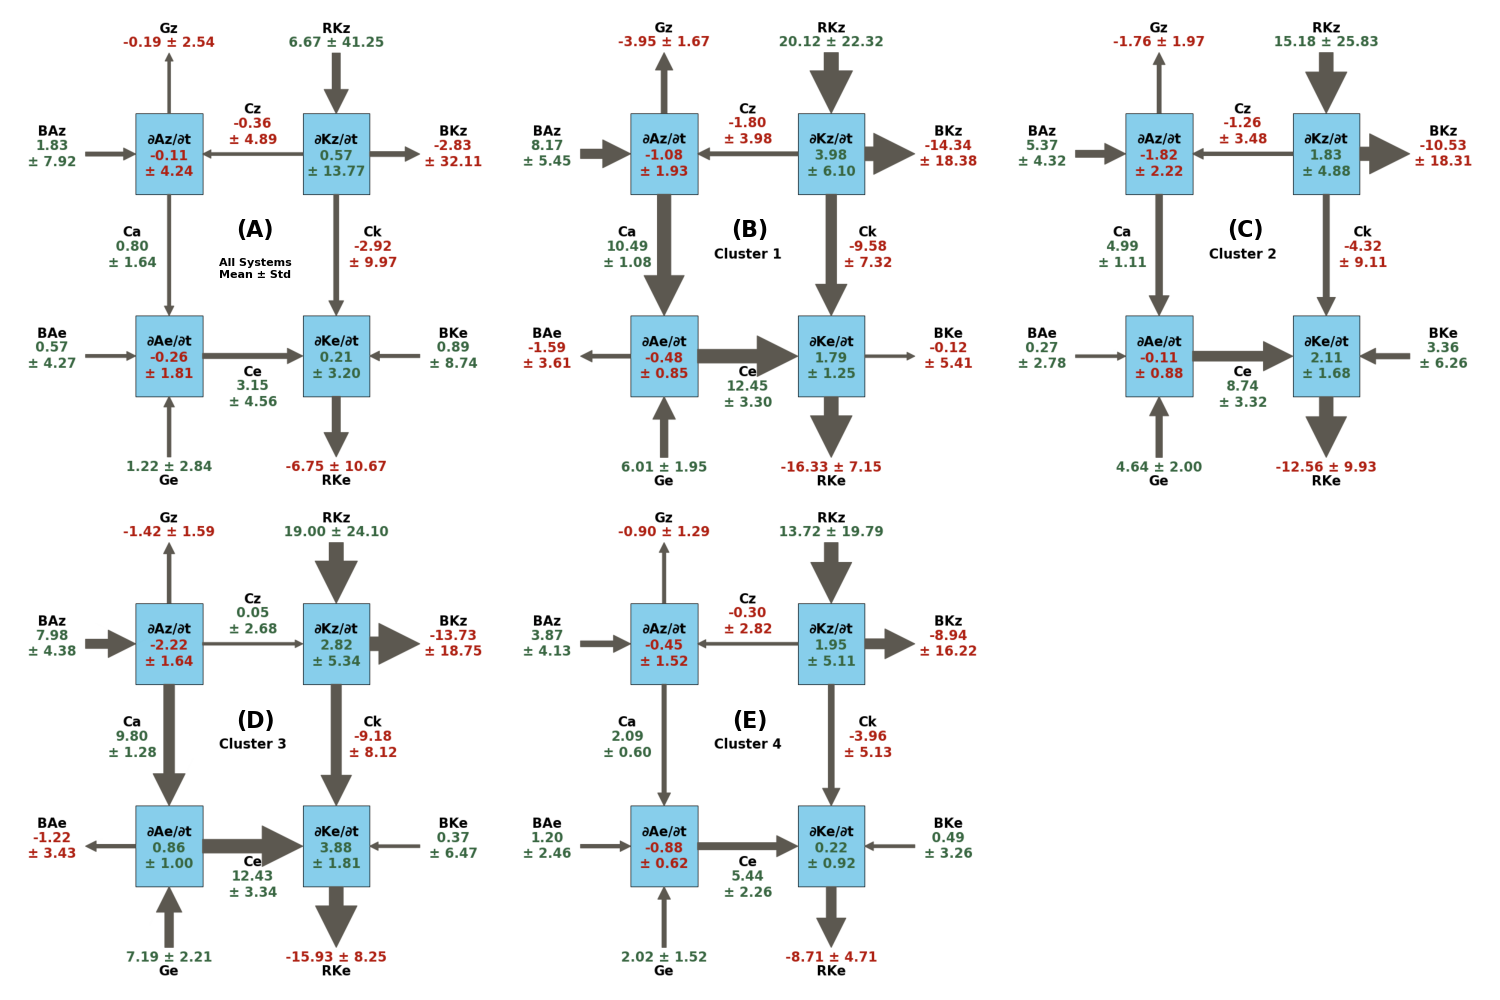
\includegraphics[width=\textwidth]{panel_LEC_clusters.png}
\caption{(A) Mean values and standard deviations of the limited-area Lorenz Energy Cycle (LEC) terms for all analyzed systems. Panels (B–F) illustrate the reconstructed LEC for the five clusters identified among the most intense cyclones in the dataset, defined as systems with maximum central relative vorticity at 850 hPa exceeding the 90th percentile.}
\label{fig:LEC_clusters_std}
\end{figure}

Comparing the energy fluxes of the clusters with the climatological mean computed across all cyclones provides insight into the mechanisms that distinguish these systems as the most intense (Figure~\ref{fig:LEC_clusters_std}). Cluster 1 exhibits a strong enhancement of the moist baroclinic chain, particularly in the \(C_A\) and \(G_E\) terms, as well as increased barotropic conversion, with both \(C_A\) and \(C_K\) contributing comparably to the \(K_E\) budget. However, imports of \(K_E\) are below average. Cluster 2 shows modest increases across all baroclinic and barotropic terms, with the highest \(K_E\) imports among all clusters. Cluster 3 displays similar proportions to Cluster 1 for \(C_A\), \(C_E\), and \(C_K\), though with slightly lower values. However, it presents the highest \(G_E\) among all clusters, and unlike Cluster 1, it exhibits positive but below-average \(K_E\) imports. Cluster 4 features the weakest energy conversions overall, despite showing nearly doubled values for baroclinic and barotropic terms relative to the full-sample average, while still presenting below-average \(K_E\) imports. Across all clusters, the residual term is not strictly proportional to the \(K_E\) budget: Cluster 1, for instance, shows the highest \(RK_E\) despite having a lower \(K_E\) budget than Clusters 2 and 3. This suggests that, although dissipation likely dominates the residual magnitude, contributions from subgrid processes and numerical errors cannot be ruled out.


Figure \ref{fig:density_panel} displays the track density for all clusters. For all clusters, the track density maxima extend from a region near the southeastern South American coast, between $30^\circ S$ and $50^\circ S$, propagating southeastward toward the Antarctic region. Cluster 2 and 3 present tracks more concentrated near the continent, related to their lower mean duration (Figure \ref{fig:duration}). In contrast, Cluster 1 presents a track maxima spread from near $60^{\circ} E$ to near $10^{\circ} E$. Meanwhile, Cluster 4 presents a maxima near the continent and other near Antarctica.  While the track density maxima near LA-PLATA and SE-BR are associated with the incipient and intensification phases of these systems, the maxima near Antarctica correspond to their decay phase \citep{couto2024new}. The relatively small displacement of these systems indicate that they might be related to explosive cyclogenesis and in fact, among explosive cyclogenesis in South America, evidence suggests a great contribution from LA-PLATA \citep{andrade2024explosive, andrade2025composite}, however, further investigation is needed to confirm this.


\begin{figure}[!htbp]
\centering
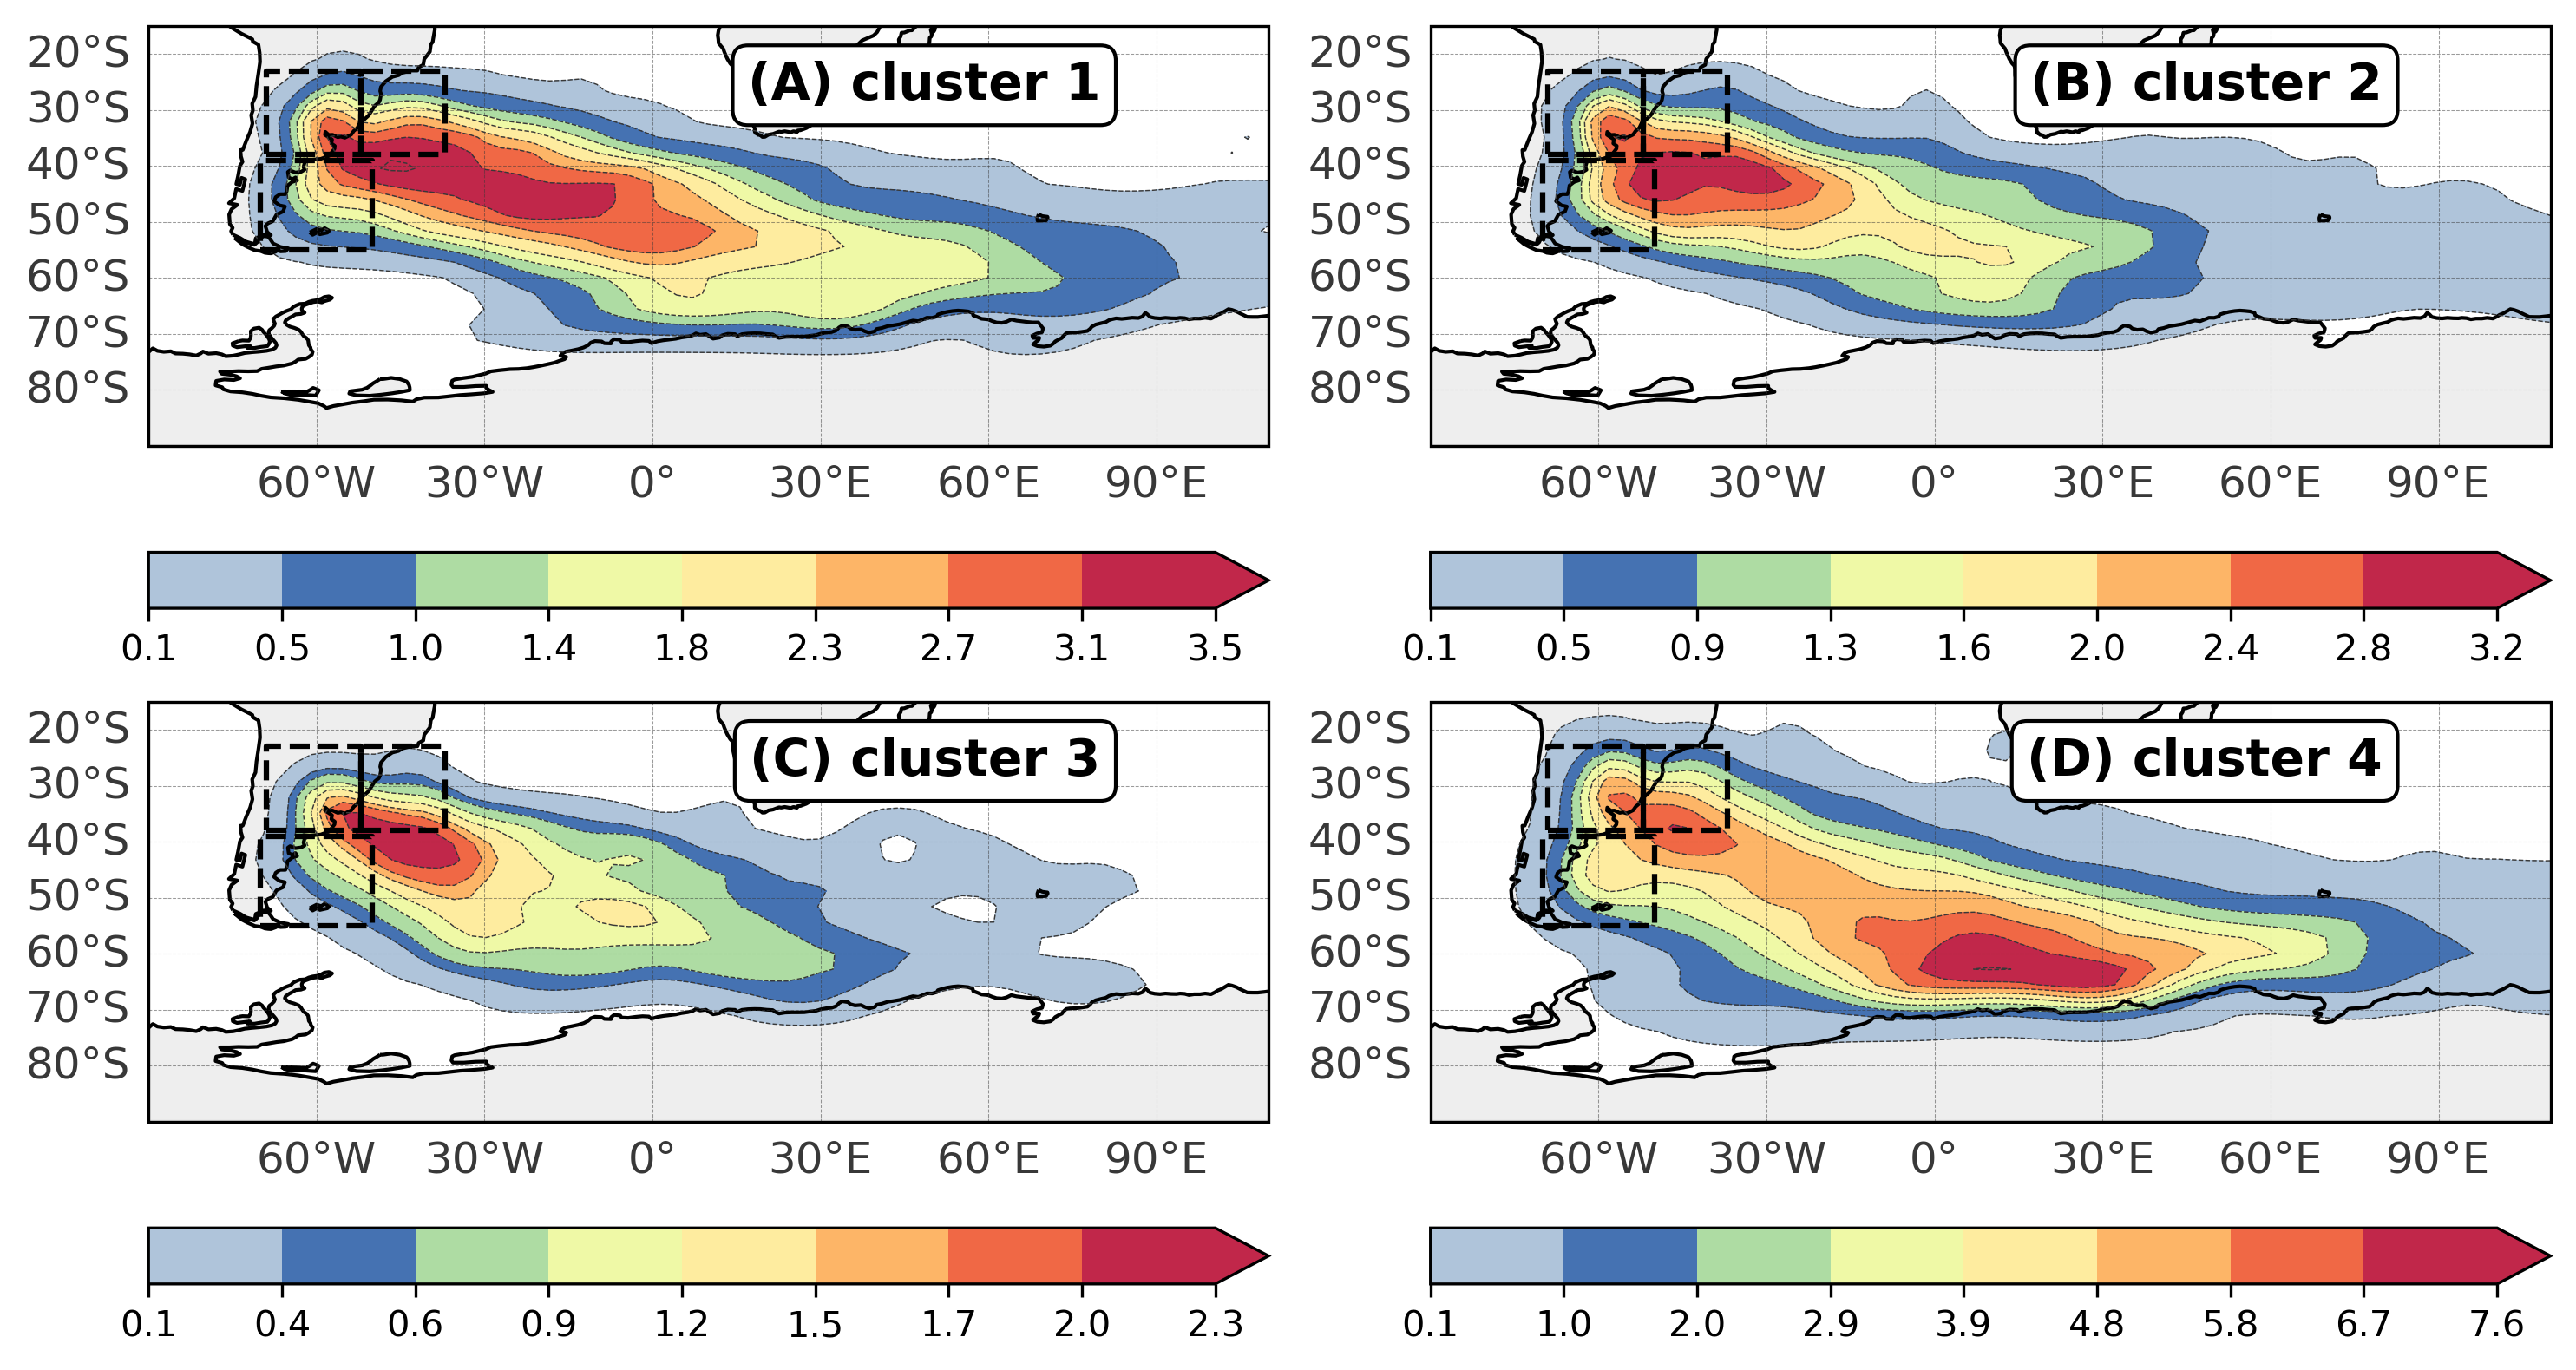
\includegraphics[width=\textwidth]{density_panel.png}
\caption{Cyclone track density for the five clusters (A–E) identified among the most intense cyclones in the dataset. These systems are defined as those with maximum central relative vorticity at 850 hPa exceeding the 90th percentile. The dashed rectangles mark the genesis regions shown in Figure \ref{fig:combined_density_map_all_phases_regions_with_regions}.}
\label{fig:density_panel}
\end{figure}

Cluster 4 has the highest number of systems (Figure~\ref{fig:cluster_analysis_panel}a), although these are generally less intense (Figure~\ref{fig:cluster_analysis_panel}b), followed by Clusters 1, 2, and 3. Cluster 3 exhibits the most intense systems on average, while Clusters 1 and 2 show similar mean intensity. Clusters 1 and 2 are more frequent during JJA, while Cluster 3 peaks in SON and Cluster 4 shows no strong seasonality (Figure~\ref{fig:cluster_analysis_panel}c). In all clusters, the proportion of cyclones originating in LA-PLATA (Figure~\ref{fig:cluster_analysis_panel}d) exceeds its baseline occurrence in the full dataset (18.9\%), reinforcing the region’s role in the development of intense systems, as noted by \citet{gramcianinov2019properties}. The seasonal distributions are also consistent with prior findings for the LA-PLATA region \citep{crespo2021potential}. The low frequency of cyclones forming in SE-BR is expected, as these tend to be weaker \citep{gramcianinov2019properties, couto2024new}. Although subtropical cyclones are most frequent over SE-BR during DJF \citep{evans2012climatology, gozzo2014subtropical}, their limited presence in this intense-cyclone subset prevents them from significantly influencing the results.


\begin{figure}[!htbp]
\centering
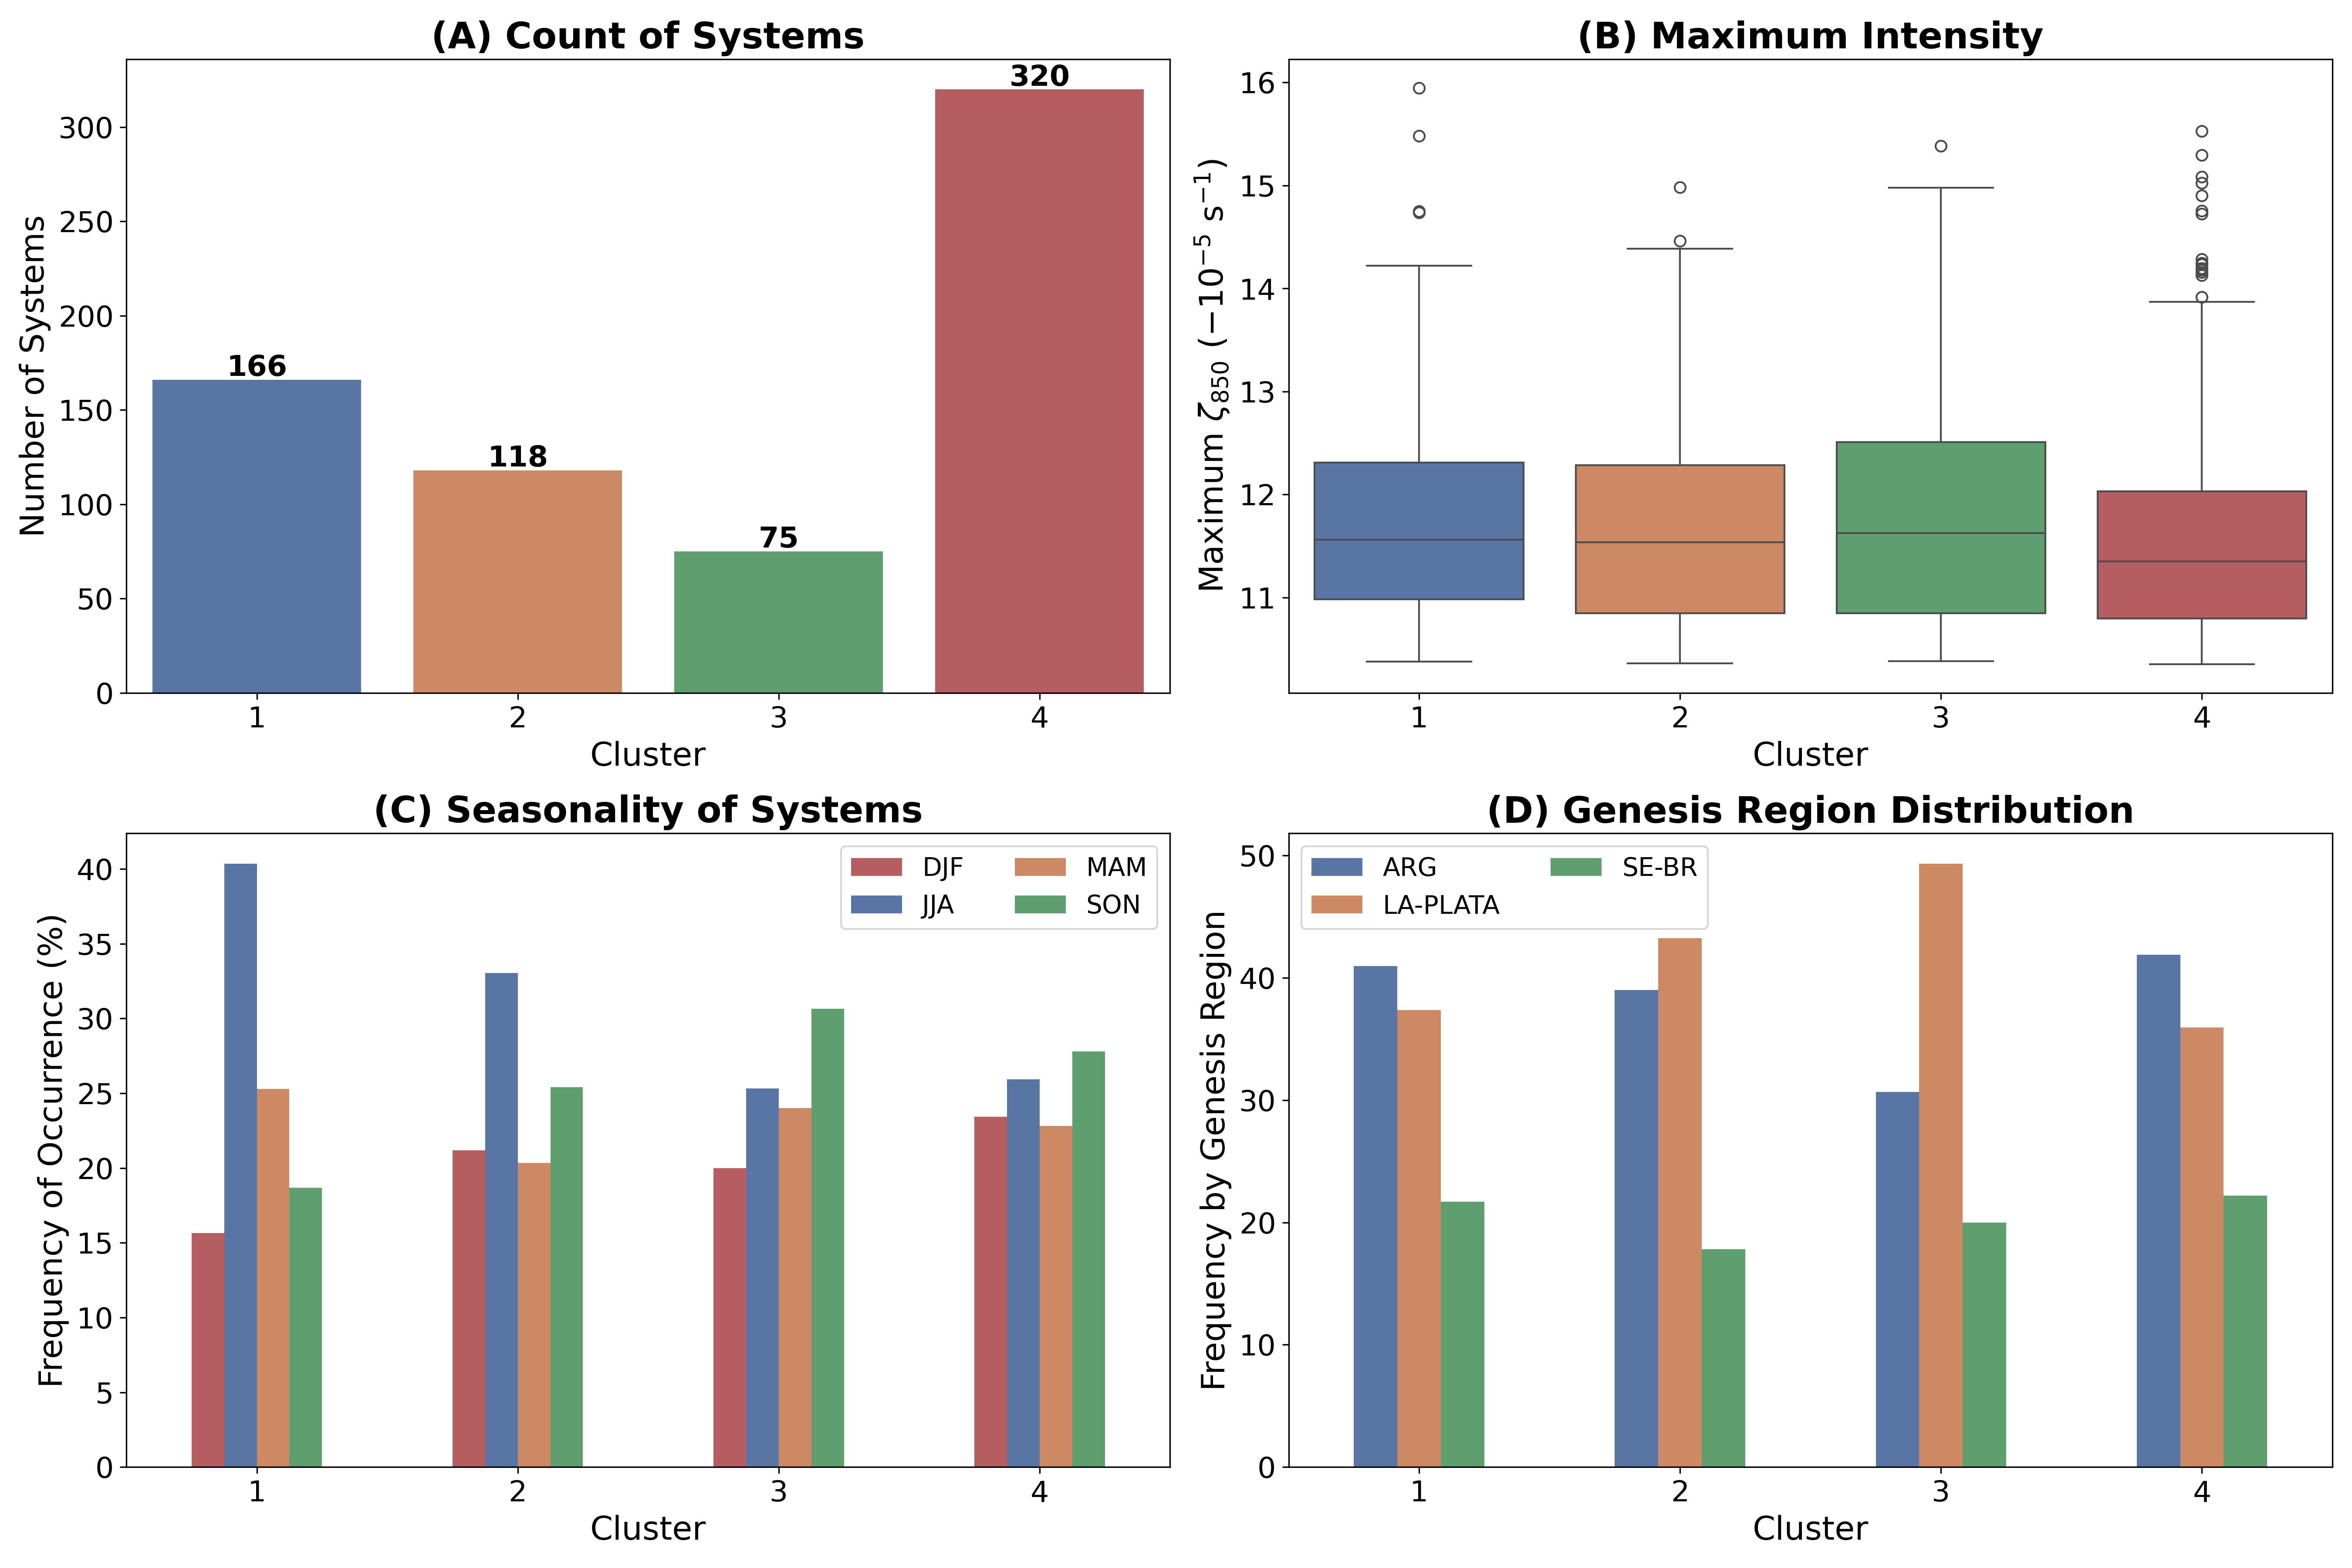
\includegraphics[width=\textwidth]{cluster_analysis_panel.png}
\caption{Characteristics of the five clusters (A–E) identified among the most intense cyclones in the dataset. (A) Number of cyclones per cluster, (B) maximum intensity (defined as maximum central relative vorticity at 850 hPa), (C) seasonal distribution of occurrences, and (D) genesis region count. In (C), colors represent different seasons (DJF, MAM, JJA, SON), while in (D), colors correspond to genesis regions (ARG, LA-PLATA, SE-BR).}
\label{fig:cluster_analysis_panel}
\end{figure}


\section{Discussion}\label{sec:discussion}

\subsection{Key Features}\label{sec:comparison}

The LEC diagrams (Figure~\ref{fig:panel_lec_mean_phases}) indicate that the mean energetic behavior is preserved across distinct life cycle phases. However, the high variability shown in Figure~\ref{fig:combined_ridge} reveals a wide range of behaviors among South Atlantic cyclones. While this section focuses on the mean energy cycle, it is important to recognize that energy budget terms serve primarily as a starting point. The energy conversions and fluxes offer more robust insight into the dynamical processes governing cyclone development. In addition to the phase-specific diagrams, a schematic of the mean Lorenz Energy Cycle for all systems is shown in Figure~\ref{fig:draw_LEC_total}, facilitating comparison across phases and highlighting dominant pathways.


\begin{figure}[!htbp]
\centering
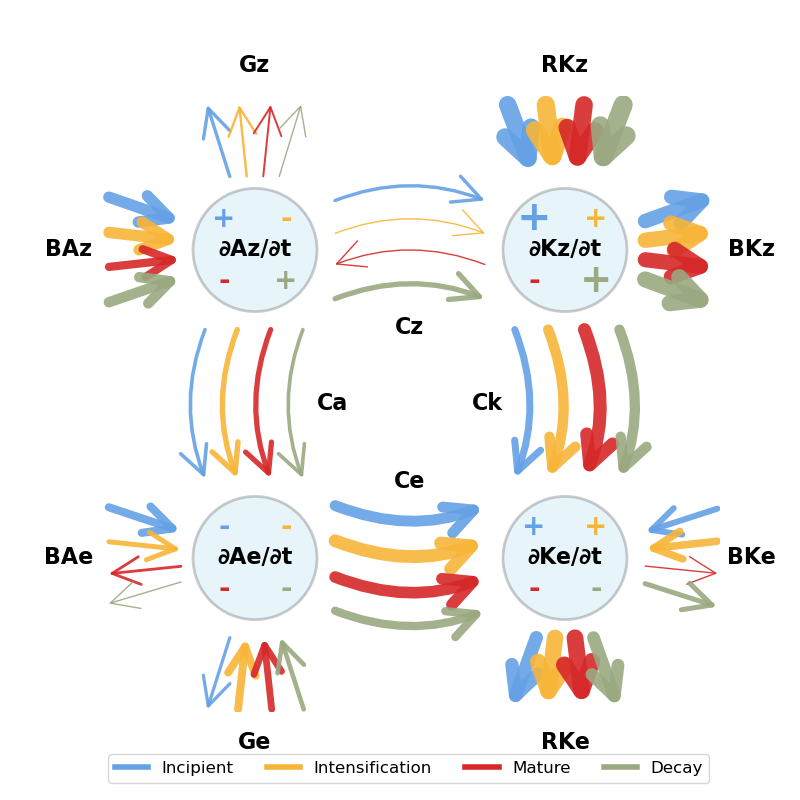
\includegraphics[width=\textwidth]{LEC_total_v6.png}
\caption{Schematic representation of the mean Lorenz Energy Cycle (LEC) for all analyzed cyclones in the South Atlantic, combining information from all life cycle phases. Arrows represent energy fluxes between reservoirs, with colors indicating the life cycle phases. The arrow thicknesses and symbol sizes for the balance terms ($\partial/\partial t$) are proportional to the absolute magnitude of each term, as presented in Figure \ref{fig:panel_lec_mean_phases}.}
\label{fig:draw_LEC_total}
\end{figure}

The $A_Z$ term increases during the early phases due to persistent influxes across the boundaries ($BA_Z > 0$), rather than local generation ($G_Z$). As baroclinic conversions intensify, the $A_Z$ budget becomes negative during the intensification and mature phases, before returning to positive in the decay phase. This evolution suggests that $A_Z$ variations are not driven by latitudinal diabatic heating contrasts. A similar pattern was reported by \citet{dias2011energy}, although their methodology excluded the incipient phase due to the use of sea-level pressure for cyclone tracking, instead of relative vorticity at 850 hPa \citep{sinclair1994objective,hoskins2002new}.

For $K_Z$, a general increase is observed except during the mature phase, when strong barotropic conversion ($K_Z \rightarrow K_E$) coincides with negative $C_Z$ values. This indicates descending motion at warmer latitudes and ascending motion at colder latitudes as the cold front reaches the equatorward side of the cyclone and the warm front reaches the poleward side. Notably, $BK_Z$ and $RK_Z$ present high magnitudes: the former suggests export of zonal kinetic energy (e.g., jet stream outflow), while the latter aggregates dissipation, boundary pressure work ($B\Phi Z$), subgrid transfers, and numerical errors. 

As the Semi-Lagrangian framework does not account for changes in the background energetics along a moving domain, part of the apparent time evolution in \(A_Z\) and \(K_Z\) may simply reflect the cyclone’s poleward drift \citep{couto2024new}. Such drift carries the system into latitudes of larger climatological background APE, implying an increase in \(A_Z\) \citep{novak2018local, liu2024systematic}. Because the zonally integrated \(K_Z\) reaches its climatological maximum near 60°\,S \citep{novak2018local, liu2024systematic}, \(K_Z\) should decrease for storms that originate over ARG and migrate poleward, but increase for those formed in SE-BR or LA-PLATA . In practice, however, both reservoirs evolve irregularly and non-monotonically, indicating that intrinsic cyclone dynamics, rather than passive domain advection, control the local energetics, corroborating \citet{federer2025synoptic}.

The $A_E$ budget is negative throughout the life cycle, with minimal values during the incipient and intensification phases. This reflects a highly active and efficient baroclinic chain. Energy is transferred from $A_Z$ via $C_A$, and from $A_E$ to $K_E$ via $C_E$, driven by meridional heat transport and vertical motions in frontal zones. During intensification, $G_E$ becomes positive, associated with convective heating along the cold front \citep[e.g.,][]{govekar2011three}. Simultaneously, radiative heating in the warm sector due to long-wave absorption from mid- to high-level clouds \citep{lau1997comparing,keshtgar2023cloud}, combined with latent heat release from intense precipitation during this phase \citep{mcerlich2023assessment}, enhances $G_E$. As the system matures and convection weakens, $BA_E$ reverses (export), and the $A_E$ budget sharply decreases. During decay, with disorganized frontal structures and weak diabatic forcing, $A_E$ returns to near-zero budget values.

The $K_E$ reservoir increases during incipient and intensification phases, as baroclinic, barotropic, and boundary fluxes supply energy. In the mature phase, barotropic conversion peaks, but weakening of baroclinic forcing and reversal of boundary fluxes, along with increased $RK_E$, lead to a net energy loss. During the decay phase, diminishing energy inputs and rising exports further reduce $K_E$. Although $RK_E$ includes numerical errors and the $B\Phi E$ term, the trend suggests dominant dissipative processes, in line with \citet{smith1980energetics}.

Both $B\Phi_Z$ and $B\Phi_E$ were directly computed and yielded large values (Table~\ref{tab:lec_stats}, Figure~\ref{fig:combined_ridge}d). These terms, representing pressure work by zonal and meridional winds at the domain boundaries, are highly sensitive to small errors in the geopotential field \citep{brennan1980zonal}. Despite quality control in ERA5, some inconsistencies may persist, and since the LECTK tool does not apply preprocessing filters, such errors likely propagate into the diagnostics. Future work should examine the physical interpretation of $B\Phi$ terms and the causes of their anomalous magnitudes, as they are seldom reported in literature.


\subsection{Cyclone Groups}

Substantial variability in the dataset, as revealed by the EOF analysis, is largely captured by EOF1(+) and EOF1(–), which together represent nearly 40\% of all systems. EOF1(+) is linked to stronger cyclones, while EOF1(–) corresponds to weaker ones (Supplementary Figure~\ref{fig:panel_2x2_metrics_q90_vs_q10}b), indicating a bi-modal structure in cyclone intensity. This suggests that "day-to-day" systems tend to follow distinct energetic regimes. Traditional cyclone climatologies over the South Atlantic tend to group all cyclones together \citep[e.g.,]{sinclair1994objective,hoskins2005new,reboita2010south,gramcianinov2019properties}. In contrast, the results presented here suggest that these systems exhibit distinct behaviors and may therefore be categorized into separate groups.


These intensity differences manifest in their energy cycles and physical characteristics. Figure~\ref{fig:EOFs_panel} presents schematic LECs for the four leading EOF(+) groups. EOF1(+) displays a consistent enhancement across all energy pathways, while EOF1(–) shows a reduction. These differences extend to cyclone mobility: EOF1(+) systems follow the South Atlantic storm track \citep{hoskins2005new,gramcianinov2019properties}, whereas EOF1(–) systems remain more confined near the South American coast (Figure~\ref{fig:density_panel_q10}a), particularly within the ARG and SE-BR regions (Figure~\ref{fig:panel_2x2_eof_statistics}d), and exhibit lower translational speeds (Figure \ref{fig:panel_2x2_metrics_q90_vs_q10}).

\begin{figure}[!htbp]
\centering
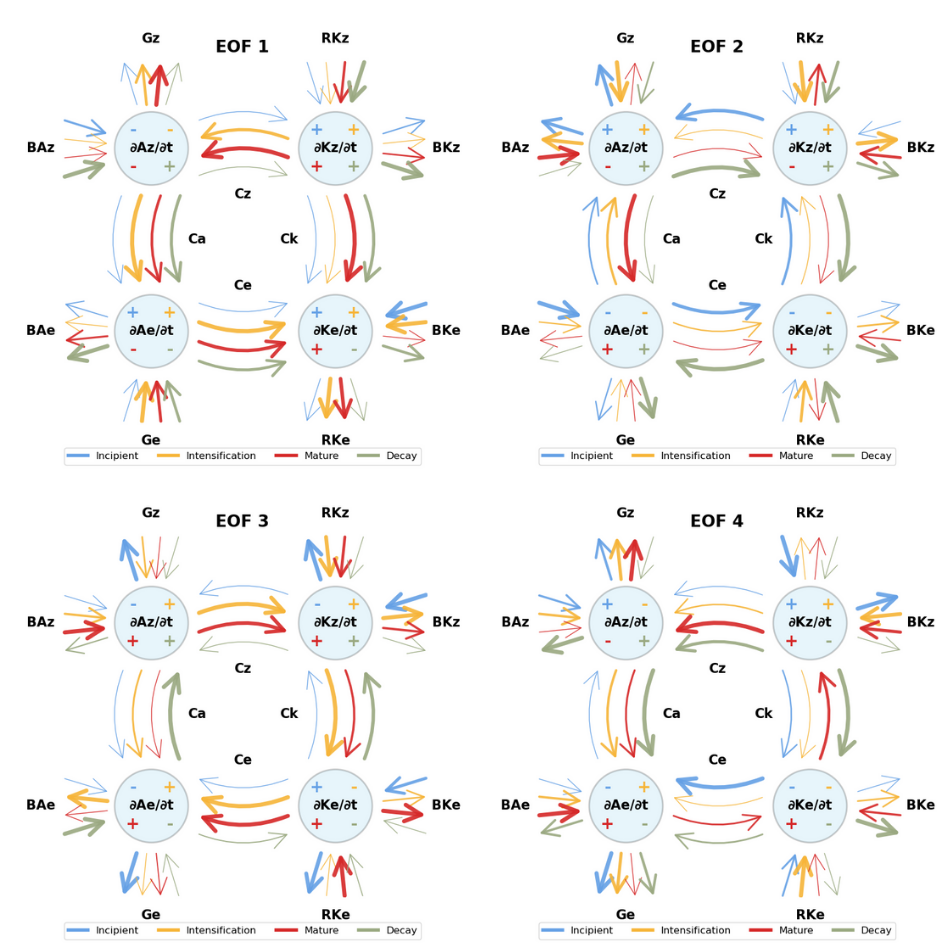
\includegraphics[width=\textwidth]{EOFs_panel.png}
\caption{Schematic representation of the mean Lorenz Energy Cycle (LEC) for cyclones associated with the four four leading positive Empirical Orthogonal Functions (EOF1(+) to EOF4(+)). Arrows represent energy fluxes between reservoirs, with colors indicating life cycle phases. The thickness of each arrow and the size of the balance terms ($\partial/\partial t$) symbols are proportional to the absolute magnitude of each term.}
\label{fig:EOFs_panel}
\end{figure}

EOF2–EOF4 describe less frequent cyclone types. EOF2(+), EOF3(–), and EOF4(–) are associated with relatively stronger systems, while their counterparts correspond to weaker ones (Figure \ref{fig:panel_2x2_metrics_q90_vs_q10}b). EOF2(+) is notable for lacking enhancements in baroclinic/barotropic conversions or \( K_E \) imports during early phases. EOF3(–) and EOF4(–), in contrast, display a pronounced intensification of the \( G_E \rightarrow A_E \rightarrow K_E \) chain, especially during the incipient and intensification phases. These patterns indicate that despite a shared dominant energy structure, South Atlantic cyclones express diverse configurations in their development. This variability is further reflected in differences in genesis region and seasonality (Figure~\ref{fig:panel_2x2_eof_statistics}), with EOF1(+) and EOF3(–) dominating among the most intense systems (Supplementary Figure~\ref{fig:intense_systems_PCs_stacked_pcs}).

For intense cyclones (above the 90th percentile in central vorticity), genesis is most frequent in LA-PLATA and during JJA—consistent with earlier studies identifying this region as favorable for strong development \citep{reboita2010south,gramcianinov2019properties,crespo2021potential}. These systems are primarily linked to moist baroclinic instability (Figure~\ref{fig:LEC_clusters_std}), particularly under the influence of a strong upper-level jet in austral winter. Meanwhile, SE-BR systems are less frequent, especially during DJF, when baroclinicity in that region is weaker \citep{gramcianinov2019properties,crespo2021potential}.

Among the four LEC-based clusters, Cluster 4 contains the largest number of systems but the lowest maximum central vorticity, making it the weakest group. Importantly, all clusters show enhanced LEC terms relative to the overall mean, reinforcing the connection between stronger energy fluxes and cyclone intensity. These findings support the robustness of the Semi-Lagrangian framework and highlight the existence of distinct energetic regimes. Even within the subset of intense cyclones, considerable diversity in energy cycle structures persists, indicating that multiple pathways can lead to strong cyclogenesis in the South Atlantic.

\subsection{Mechanisms of Energy Transfer}

Throughout this study, barotropic conversions ($C_K$) emerged as a key mechanism for cyclone development in the South American region. While extratropical cyclones are traditionally associated with baroclinic instability \citep{bjerknes1922life,charney1964growth,hoskins1990existence}, our results show that moist baroclinic processes dominate during the intensification phase, whereas barotropic conversions peak during the mature stage (Figure~\ref{fig:panel_lec_mean_phases}). Notably, $C_K$ magnitudes are nearly three times larger than those of $C_A$, suggesting a stronger contribution from zonal kinetic energy to eddy development than from meridional temperature gradients.

Despite LEC-based studies dating back decades, few have examined South Atlantic cyclones, limiting direct comparisons. Case studies on tropical systems emphasize the $G_E \rightarrow A_E \rightarrow K_E$ chain and barotropic conversions \citep{brennan1980zonal,veiga2008analysis}, while subtropical systems show mixed roles for both baroclinic and barotropic conversions \citep{michaelides1987limited,dias2013synoptic,pezza2014large,cavicchia2018energetics}. For extratropical systems, energy pathways vary: some are baroclinically dominated \citep{dias2011energy,black2013universal}, others barotropically \citep{michaelides1992spatial,dias2011energy}, and some combine both with varying degrees of $K_E$ import \citep{wahab2002mechanism,bulic2006limited,pezza2010environmental}. Thus, although the relevance of barotropic instability in extratropical cyclones is not novel, this work provides the first large-sample LEC analysis for the South Atlantic, offering a consolidated view of this behavior. These findings are consistent with recent studies that link storm track intensification in the Southern Hemisphere to enhanced barotropic growth \citep{chemke2022intensification}, associate storm growth time with barotropic conversion \citep{hadas2025lagrangian}, and identify barotropic conversions from $K_Z$ to $K_E$ within storm track regions \citep{liu2024systematic}.

It is also important to emphasize that, while previous studies investigated the LEC using an Eulerian framework, this study employed a Semi-Lagrangian framework. This approach has the advantage of isolating the energetics strictly related to the target system. However, the extent to which this methodology differs from the Eulerian framework in representing the magnitude and direction of energy fluxes has not been extensively assessed, apart from one study by \citet{michaelides1999quasi}. Also, the extent to which our findings generalize to other regions remains uncertain. Given the stronger jets and meridional wind gradients in the Southern Hemisphere \citep[e.g.,][]{swart2019canadian,jain2023monsoon,savita2023assessment}, barotropic conversions may be more pronounced in the South Atlantic than in the North Atlantic—a hypothesis requiring further study.

Another distinction is found in the decay phase. While most previous studies report $K_E \rightarrow K_Z$ conversions during cyclone decay \citep[e.g.,][]{dias2011energy,veiga2008analysis,pezza2014large}, this pattern was not observed here. In our analysis, the decay phase, the longest for these systems \citep{couto2024new}, is averaged over multiple timesteps and features $C_K$ values that gradually shift from strongly negative in the mature phase to near neutral at the end of the lifecycle (Figures~\ref{fig:panel_lec_mean_phases}C and \ref{fig:ck_decay_phase_median_iqr}). This suggests that barotropic conversion continues to sustain the system during decay, until dissipation dominates. Prior use of large Eulerian domains may have underestimated $C_K$, as seen in \citet{black2013universal}, where $C_K$ remains positive across all phases.

Some limitations of our approach must be acknowledged. Although the Semi-Lagrangian framework follows the cyclone's trajectory, it does not account for regional variations in background APE and kinetic energy. This may influence $A_Z$, $K_Z$, and their boundary terms as the system moves through varying energy environments. Furthermore, the LEC formulation relies on a global reference state for APE. In contrast, the local APE framework proposed by \citet{novak2018local} defines APE relative to each air parcel’s individual reference state. While this approach can yield additional insights—such as the potential for cyclones to locally generate APE \citep{federer2024local}, the overall global energy fluxes remain consistent between the global and local formulations \citep{liu2024systematic}. Moreover, the modest $BA_Z$ values observed here (Figure~\ref{fig:panel_lec_mean_phases}) may be partially explained by APE transport from the polar upper troposphere, as shown for the North Atlantic storm tracks by \citet{federer2025synoptic}.

\section{Summary and Conclusions}\label{sec:conclusion}

In this study, we examined the Lorenz Energy Cycle (LEC) for 6,789 cyclonic systems originating in the Southwestern Atlantic, presenting what is, to the best of our knowledge, the first comprehensive climatology of cyclones' energy cycles in this region. A notable exception is the work by \citet{black2013universal}, which focused solely on explosive cyclones and used large fixed domains, contrasting with the Semi-Lagrangian approach adopted in this study. While studies such as \citet{smith1980energetics} provide valuable reviews of the energetics of extratropical cyclones, focusing on broad averages and generalized mechanisms, and case studies have explored the dynamics of specific systems \citep[e.g.]{pezza2014large,dias2011energy,cavicchia2018energetics}, our study adopts a climatological approach. Specifically, we track the energy cycles of individual cyclones across distinct life cycle phases, offering a more detailed investigation of the unique physical mechanisms that drive energy conversions in this region. Furthermore, the use of the Cyclophaser program to dissect the life cycles of cyclones has enabled a novel investigation of the energy cycle across different developmental stages, providing deeper insights into the variability and dynamism of these systems.

The results presented here demonstrate that, for most cyclonic systems in the South Atlantic, a clear pattern of energy flow is evident. This pattern is characterized by both barotropic and baroclinic conversions providing energy for eddy development and is preserved throughout the cyclone life cycle phases, despite variations in magnitude. Barotropic conversions tend to be 2 to 3 times larger in magnitude than baroclinic conversions, with the former peaking during the mature phase and the latter during the intensification phase. The generation of eddy potential energy and the imports of eddy kinetic energy play secondary roles. The former peaks during the intensification phase and remains positive through the mature and decay phases, while the latter occurs primarily during the incipient (cyclogenesis) and intensification phases.

Despite the high variability among the systems, the EOF analysis indicates that, in most cases, the main behavior is preserved. This variability is instead expressed as a strengthening and/or weakening of specific energy pathways, indicating that cyclonic development in the South Atlantic region can be attributed to distinct dynamical processes, as supported by the literature. Consequently, it is possible to hypothesize that these systems can be grouped into distinct types based on their characteristics and energy cycles. This heterogeneity is also evident among the most intense systems. For these systems, distinct groups exhibit varying relative contributions of energy from barotropic and baroclinic chains, as well as differences in eddy generation of APE and imports of eddy kinetic energy. Although most of these intense systems originate in the LA-PLATA region, the variability in the relative proportions of genesis regions among the different clusters is reflected in their energy cycles and mean characteristics.

The goal of this study was to investigate the energy cycle of cyclones in the South Atlantic region using a Semi-Lagrangian approach. As a pioneering study of this kind, several questions have emerged throughout its development. For instance, previous studies for this region have assessed the distinct synoptic and dynamical conditions related to cyclogenesis in the three primary genesis regions, as well as the seasonal variability in their development \citep{gramcianinov2019properties, crespo2021potential}. A distinction in the energy cycles among these genesis regions, along with their seasonal variability, would therefore be valuable. Additionally, given the prominence of barotropic conversions as an energy source for cyclone development, the question arises as to whether barotropic instability is truly occurring near the cyclone center. \citet{souza2024thesis} proposed a framework for classifying cyclones into distinct groups based on their energy cycles. In an upcoming study, this method will be applied to address these questions and further investigate these topics.


\backmatter


%TC:ignore

\section*{Appendix}


Mathematical expressions used for the calculation of the Lorenz Energy Cycle (LEC), adopting the notation from \citet{michaelides1987limited}. 


Firstly, we define the zonal mean of a variable $X$, between longitudes $\lambda_{1}$ and $\lambda_{2}$:

 \begin{equation}
     [X]_\lambda = \frac{1}{\lambda_2 - \lambda_1} \int_{\lambda_2}^{\lambda_1} X d\lambda
 \end{equation}

The eddy component of this variable is its deviation from the zonal mean:

\begin{equation}
    (X)_\lambda =  X - [X]_\lambda
\end{equation}

The domain mean of the variable $X$, defined over the computational domain bounded by longitudes $\lambda_1$ and $\lambda_2$, and latitudes $\phi_1$ and $\phi_2$, is given by:

\begin{equation}
    [X]_{\lambda\phi} = \left(\frac{1}{\lambda_2 - \lambda_1}\right)  \left(\frac{1}{\sin\phi_2 - \sin\phi_1}\right) \int_{\lambda_2}^{\lambda_1} X cos\phi d\lambda d\phi 
\end{equation}

Similarly, we define the deviation of the zonal mean from the domain mean:

\begin{equation}
    ([X]_\lambda)_\phi = [X]_\lambda - [X]_{\lambda\phi}
\end{equation}

From the definitions above, the four energy components used in the LEC computation are defined as follows:

\begin{align}
   &A_Z = \int_{p_t}^{p_b} \frac{[{([T]_\lambda)_\phi}^{2}]_{\lambda \phi}}  {2[\sigma]_{\lambda \phi}} dp \label{eq:AZ} \\
   &A_E = \int_{p_t}^{p_b} \frac{[{(T)_\lambda}^{2}]_{\lambda \phi}}  {2[\sigma]_{\lambda \phi}} dp \label{eq:AE} \\
   &K_Z =  \int_{p_t}^{p_b} \frac{[{[u]_\lambda}^2 + {[v]_\lambda}^2]_{\lambda \phi}}{2g} dp \label{eq:KZ} \\
   &K_E =  \int_{p_t}^{p_b} \frac{{[(u)_\lambda}^2 + {(v)_\lambda}^2]_{\lambda \phi}}{2g} dp \label{eq:KE}
\end{align}

where $p$ is the atmospheric pressure, with subscripts $b$ and $t$ denoting the lower (base) and upper (top) pressure boundaries of the atmosphere, respectively. $T$ represents temperature, $g$ is the acceleration due to gravity, and $u$ and $v$ are the zonal and meridional wind components, respectively. The static stability parameter $\sigma$ is defined as:


\begin{equation}
    \sigma = \left[\frac{gT}{c_p}-\frac{pg}{R}\frac{\partial T}{\partial p}\right]_{\lambda \phi}
\end{equation}

where $c_p$ is the specific heat at constant pressure, and $R$ is the ideal gas constant for dry air.


The four conversion terms are defined as follows, integrating over the atmospheric column from the base ($p_b$) to the top ($p_t$) pressures:


\begin{align}
    &C_Z = \int_{p_t}^{p_b} - [\left([T]_\lambda)_\phi ([\omega]_\lambda\right)_\phi]_{\lambda\phi} \ \frac{R}{gp} \ dp \label{eq:CZ} \\
    &C_E = \int_{p_t}^{p_b} - [(T)_\lambda (\omega)_\lambda]_{\lambda\phi} \ \frac{R}{gp} \ dp \label{eq:CE} \\
    &C_A = \int_{p_t}^{p_b} - \left( \frac{1}{2a\sigma}  \left[ (v)_\lambda (T)_\lambda  \frac{\partial  ([T]_\lambda)_\phi}{\partial \phi} \right]_{\lambda\phi} + \frac{1}{\sigma}  \left[ (\omega)_\lambda (T)_\lambda \frac{\partial  ([T]_\lambda)_\phi}{\partial p} \right]_{\lambda\phi} \right) dp \label{eq:CA} \\
    \begin{split} &C_K = \int_{p_t}^{p_b} \frac{1}{g} \left(
    \left[ \frac{\cos\phi}{a} (u)_\lambda (v)_\lambda \frac{\partial}{\partial\phi} \left(\frac{[u]_\lambda}{\cos\phi}\right)\right]_{\lambda\phi} + \left[ \frac{{(v)_\lambda}^2}{a} \frac{\partial [v]_\lambda}{\partial\phi}  \right]_{\lambda\phi}  \right. \\
    &\left. + \left[ \frac{\tan\phi}{a} {(u)_\lambda}^2 [v]_\lambda  \right]_{\lambda\phi} + \left[ (\omega)_\lambda  (u)_\lambda \frac{\partial [u]_\lambda}{\partial p} \right]_{\lambda\phi} + \left[ (\omega)_\lambda  (v)_\lambda \frac{\partial [v]_\lambda}{\partial p} \right]_{\lambda\phi}  \right) dp \end{split} \label{eq:CK}
\end{align}

where $a$ is the Earth's radius and $\omega$ is the vertical velocity in isobaric coordinates. 


The APE generation and K dissipation terms are defined as:

\begin{align}
    &G_Z =  \int_{p_t}^{p_b} \frac{[([q]_\lambda)_\phi ([T]_\lambda)_\phi]_{\lambda \phi}}{c_p[\sigma]_{\lambda \phi}} dp \\
    &G_E =  \int_{p_t}^{p_b} \frac{[(q)_\lambda (T)_\lambda]_{\lambda \phi}}{c_p[\sigma]_{\lambda \phi}} dp \\
    &D_Z = -  \int_{p_t}^{p_b} \frac{1}{g} [[u]_\lambda [F_\lambda]_\lambda + [v]_\lambda [F_\phi]_\lambda]_{\lambda \phi} dp \\
    &D_E = -  \int_{p_t}^{p_b} \frac{1}{g} [(u)_\lambda (F_\lambda)_\lambda + (v)_\lambda (F_\phi)_\lambda]_{\lambda \phi} dp
\end{align}

Here, $F_{\lambda}$ and $F_{\phi}$ represent the zonal and meridional frictional components, respectively, and $q$ is the diabatic heating term, computed as a residual from the thermodynamic equation:

\begin{equation}
    \frac{q}{c_p} = \frac{\partial T}{\partial t} - \Vec{V}_H \cdot \Vec{\nabla}_p T - S_p\omega
\end{equation}

where $-\Vec{V}_H \cdot \Vec{\nabla}_p T$ represents the horizontal advection of temperature and $S_p$ approximates the static stability, given by:

\begin{equation}
    S_p \equiv -\frac{T}{\theta}\frac{\partial \theta}{\partial p}
\end{equation}

where $\theta$ is the potential temperature. 


The boundary terms are given by:

\begin{align}
& \mathrm{BAZ}=c_1 \int_{p_1}^{p_2} \int_{\varphi_1}^{\varphi_2} \frac{1}{2[\sigma]_{\lambda_{\varphi}}}\left(2\left([T]_\lambda\right)_{\varphi}(T)_\lambda u+{\left([T]_{\lambda_{\varphi}}\right)_{\varphi}}^2 u\right)_{\lambda_1}^{\lambda_2} \nonumber \\
& \times d \varphi d p+c_2 \int_{p_1}^{p_2} \frac{1}{2[\sigma]_{\lambda \varphi}}\left(2\left[(v)_\lambda(T)_\lambda\right]_\lambda\left([T]_\lambda\right)_{\varphi} \cos \varphi \right. \left.+{\left([T]_\lambda\right)_{\varphi}}^2[v]_\lambda \cos \varphi\right)_{\varphi_1}^{\varphi_2} d p \nonumber \\
& -\frac{1}{2[\sigma]_{\lambda \varphi}}\left(\left[2(\omega)_\lambda(T)_\lambda\right]_\lambda\left([T]_\lambda\right)_{\varphi}+\left[[\omega]_\lambda{\left([T]_\lambda\right)_{\varphi}}^2\right]_{\lambda_{\varphi}}\right)_{p_1}^{p_2} \\
& \mathrm{BAE}=c_1 \int_{p_1}^{p_2} \int_{\varphi_1}^{\varphi_2} \frac{1}{2[\sigma]_{\lambda \varphi}}\left[u{(T)_\lambda}^2\right]_{\lambda_1}^{\lambda_2} d \varphi d p \nonumber \\
& +c_2 \int_{p_1}^{p_2} \frac{1}{2[\sigma]_{\lambda \varphi}}\left(\left[{(T)_\lambda}^2 v\right]_\lambda \cos \varphi\right)_{\varphi_1}^{^{\varphi_2}} d p \\
& -\left(\frac{\left[\omega{(T)_\lambda}^2\right]_{\lambda \varphi}}{2[\sigma]_{\lambda \varphi}}\right)_{p_1}^{p_2} \nonumber \\
& \mathrm{BKZ}=c_1 \int_{p_1}^{p_2} \int_{\varphi_1}^{\varphi_2} \frac{1}{2 g}\left(u\left[u^2+v^2-{(u)_\lambda}^2-{(v)_\lambda}^2\right]\right)_{\lambda_1}^{\lambda_2} \nonumber \\
& \times d \varphi d p+c_2 \int_{p_1}^{p_2} \frac{1}{2 g}\left(\left[v \cos \varphi \left[u^2+v^2\right.\right.\right. \left.\left.-{(u)_\lambda}^2-{(v)_\lambda}^2\right]\right]_{\varphi_1}^{\varphi_2} d p  \\
& -\left(\frac{1}{2 g}\left[\omega\left[u^2+v^2-{(u)_\lambda}^2-{(v)_\lambda}^2\right]\right]_{\lambda \varphi}\right)_{p_1}^{p_2} \nonumber \\
& \mathrm{BKE}=c_1 \int_{p_1}^{p_2} \int_{\varphi_1}^{\varphi_2} \frac{1}{2 g}\left(u\left[{(u)_\lambda}^2+{(v)_\lambda}^2\right]\right)_{\lambda_1}^{\lambda_2} d \varphi d p \nonumber \\
& +c_2 \int_{p_1}^{p_2} \frac{1}{2 g}\left(\left[v \cos \varphi\left[{(u)_\lambda}^2+{(v)_\lambda}^2\right]\right]_\lambda\right)_{\varphi_1}^{\varphi_2} d p \\
& -\left(\frac{1}{2 g}\left[\omega\left[{(u)_\lambda}^2+{(v)_\lambda}^2\right]\right]_{\lambda \varphi}\right)_{p_1}^{p_2} \nonumber
\end{align}

where $c_1=-\left[a\left(\lambda_2-\lambda_1\right)\left(\sin \varphi_2-\sin \varphi_1\right)\right]^{-1}, c_2=-[a$ $\left.x\left(\sin \varphi_2-\sin \varphi_1\right)\right]^{-1}$.


Lastly, the terms $B\Phi Z$ and $B\Phi E$ are given by:

\begin{align}
\mathrm{B} \Phi \mathrm{Z}= & c_1 \int_{p_1}^{p_2} \int_{\varphi_1}^{\varphi_2} \frac{1}{g}\left([v]_\lambda\left([\Phi]_\lambda\right)_{\varphi}\right)_{\lambda_1}^{\lambda_2} d \varphi d p \nonumber \\
& +c_2 \int_{p_1}^{p_2} \frac{1}{g}\left(\cos \varphi[v]_\lambda\left([\Phi]_\lambda\right)_{\varphi}\right)_{\varphi_1}^{\varphi_2} d p  \\
& -\frac{1} {g}\left(\left[\left([\omega]_\lambda\right)_{\varphi}\left([\Phi]_\lambda\right)_{\varphi}\right]_{\lambda_{\varphi}}\right)_{p_1}^{p_2} \nonumber \\
\mathrm{~B} \Phi \mathrm{E}= & c_1 \int_{p_1}^{p_2} \int_{\varphi_1}^{\varphi_2} \frac{1}{g}\left((u)_\lambda(\Phi)_{\lambda_\lambda}\right)_{\lambda_1}^{\lambda_2} d \varphi d p \nonumber \\
& +c_2 \int_{p_1}^{p_2} \frac{1}{g}\left(\left[(v)_\lambda(\Phi)_{\lambda_\lambda}\right]_\lambda \cos \varphi\right)_{\varphi_1}^{\varphi_2} d p \\
& -\frac{1}{g}\left(\left[(\omega)_\lambda(\Phi)_\lambda\right]_{\lambda_{\varphi}}\right)_{p_1}^{p_2} \nonumber
\end{align}

\section*{Declarations}

\subsection*{Funding}

This study was partly financed by the Coordenação de Aperfeiçoamento de Pessoal de Nível Superior – Brasil (CAPES) under Finance Code 001.

\subsection*{Competing interests}

The authors have no relevant financial or non-financial interests to disclose.

\subsection*{Data Availability}

The cyclone tracks used in this study were obtained from the \textit{Atlantic Extratropical Cyclone Tracks Database}, available at \url{https://doi.org/10.17632/kwcvfr52hp.4}. All datasets, including the computed Lorenz Energy Cycle results for each cyclone, along with the scripts used to generate the figures and analyses presented in this study, are publicly available at the following GitHub repository: \url{https://github.com/daniloceano/energetic_patterns_cyclones_south_atlantic}. The source code of the \texttt{Cyclophaser} package, used for detecting cyclone life cycle phases, is available on PyPI at \url{https://pypi.org/project/cyclophaser/}. The \texttt{LorenzCycleToolkit} package, used for computing the Lorenz Energy Cycle components, is also available on PyPI at \url{https://pypi.org/project/LorenzCycleToolkit/}.

\subsection*{Author contributions}

Conceptualization: Danilo Couto de Souza, Pedro Leite da Silva Dias, Ricardo de Camargo, Carolina Barnez Gramcianinov; Methodology: Danilo Couto de Souza, Pedro Leite da Silva Dias, Ricardo de Camarg; Formal analysis and investigation: Danilo Couto de Souza, Pedro Leite da Silva Dias; Writing - original draft preparation: Danilo Couto de Souza; Writing - review and editing: Danilo Couto de Souza, Pedro Leite da Silva Dias, Ricardo de Camargo, Carolina Barnez Gramcianinov; Funding acquisition: Pedro Leite da Silva Dias, Ricardo de Camargo; Resources: Pedro Leite da Silva Dias, Ricardo de Camargo; Supervision: Pedro Leite da Silva Dias, Ricardo de Camargo.

\bibliography{sn-bibliography}% common bib file
%% if required, the content of .bbl file can be included here once bbl is generated
%%\input sn-article.bbl

\section*{Supplementary information}

\renewcommand{\thefigure}{S\arabic{figure}}
\setcounter{figure}{0}

\begin{figure}[!htbp]
    \centering
    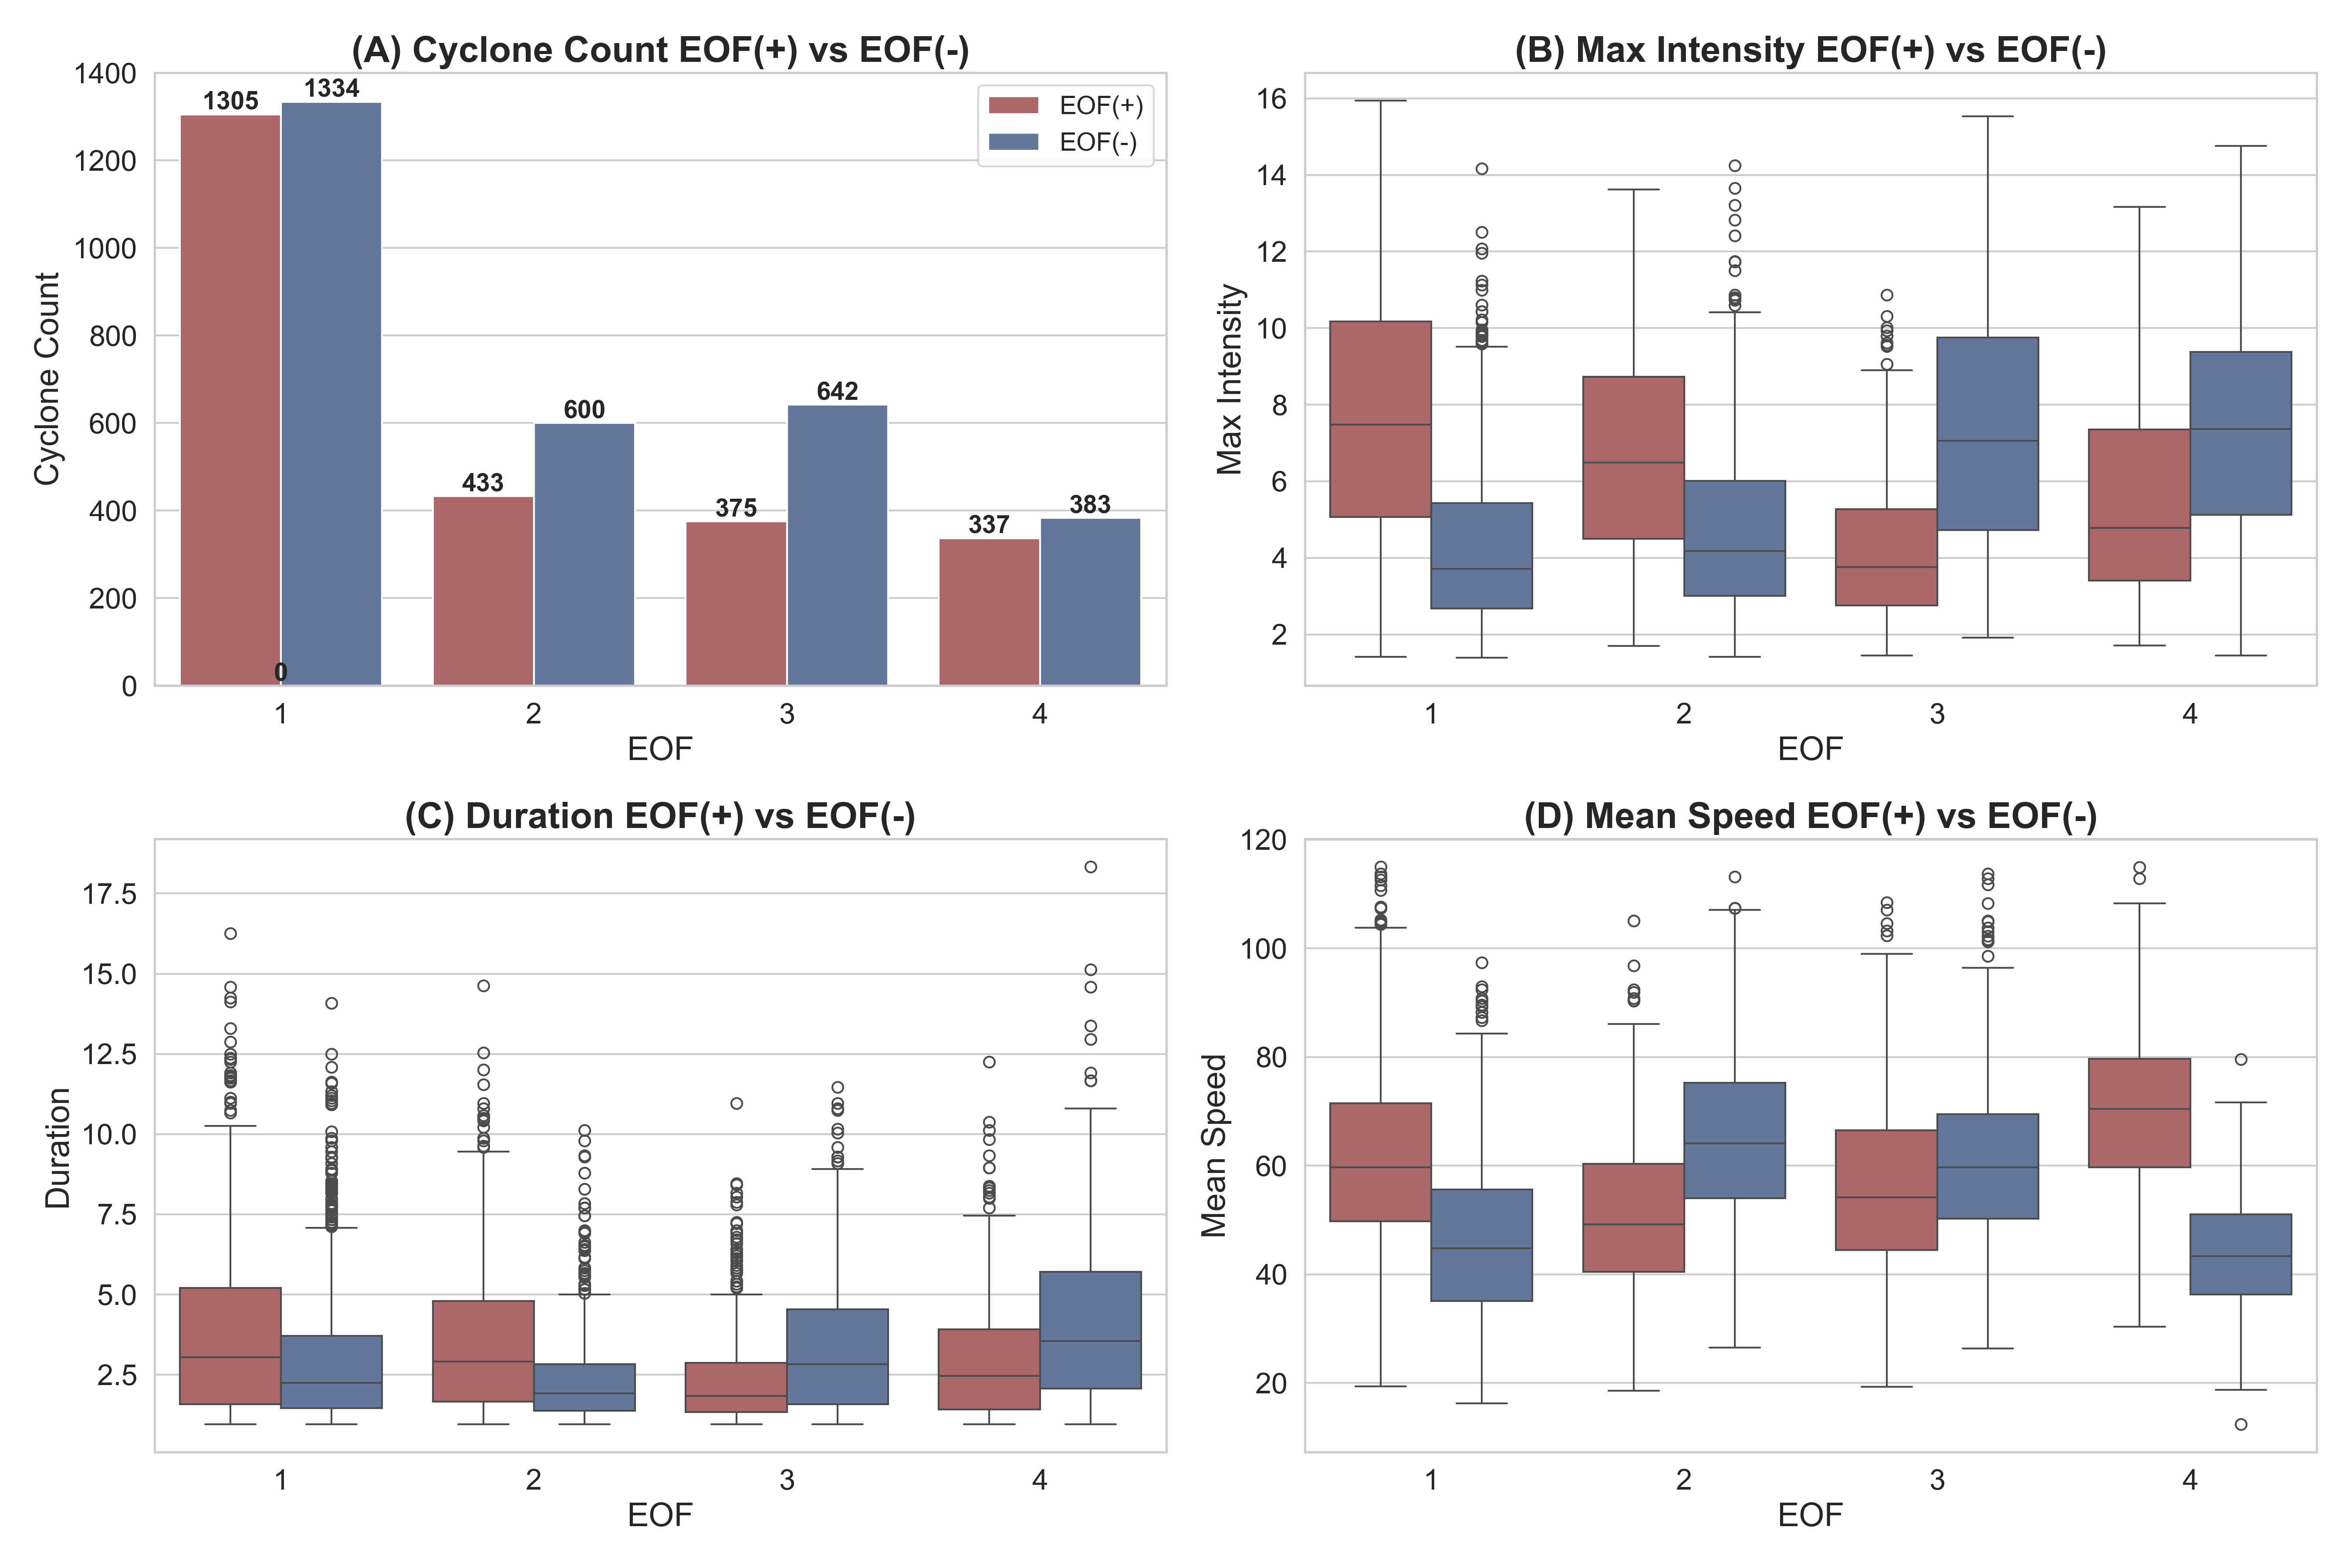
\includegraphics[width=\textwidth]{panel_2x2_metrics_q90_vs_q10.png}
    \caption{Statistics for the cyclones classified as EOF(\,+) (red) and EOF(\,$-$) (blue). 
    (A)~Cyclone counts; 
    (B)~maximum intensity, expressed by the \emph{minimum} central relative vorticity at 850\,hPa; 
    (C)~total life-cycle duration (days); and 
    (D)~mean translational speed (km\,h$^{-1}$).}
    \label{fig:panel_2x2_metrics_q90_vs_q10}
\end{figure}

\begin{figure}[!htbp]
    \centering
    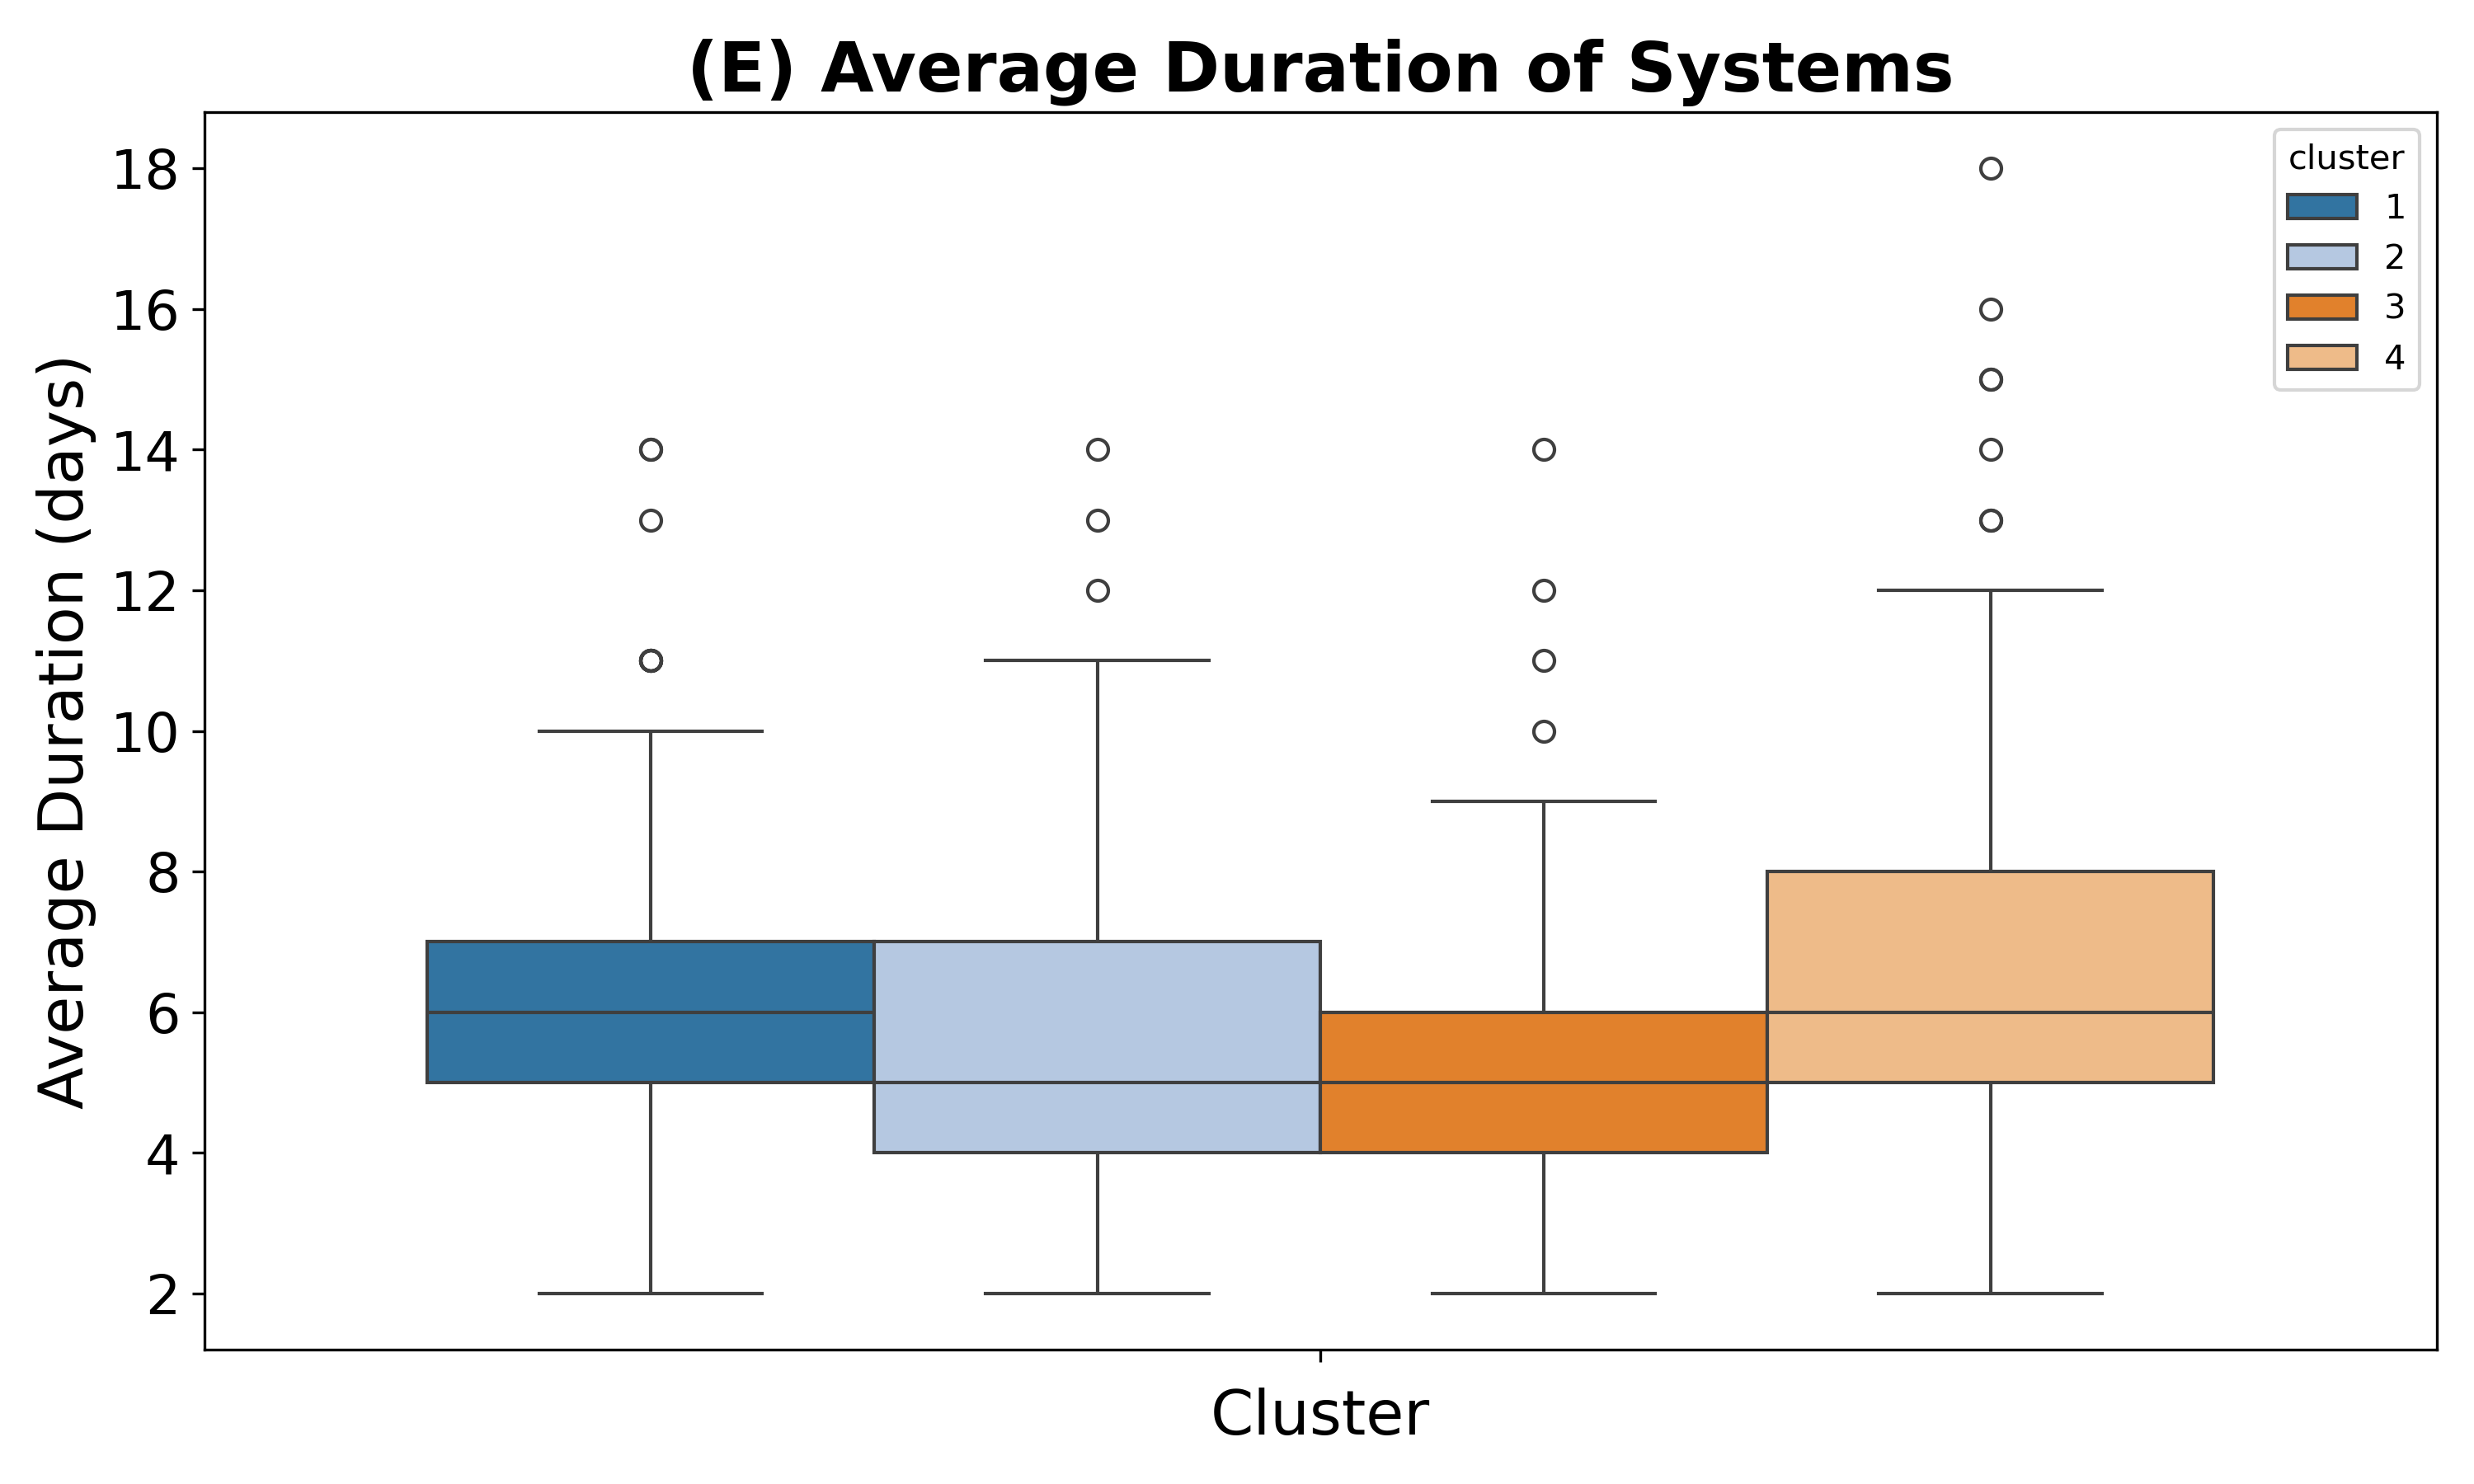
\includegraphics[width=\textwidth]{duration.png}
    \caption{Boxplot of the total life cycle duration (in days) for the four clusters (1–4) identified among the most intense cyclones in the dataset.}
    \label{fig:duration}
\end{figure}

\begin{figure}[!htbp]
    \centering
    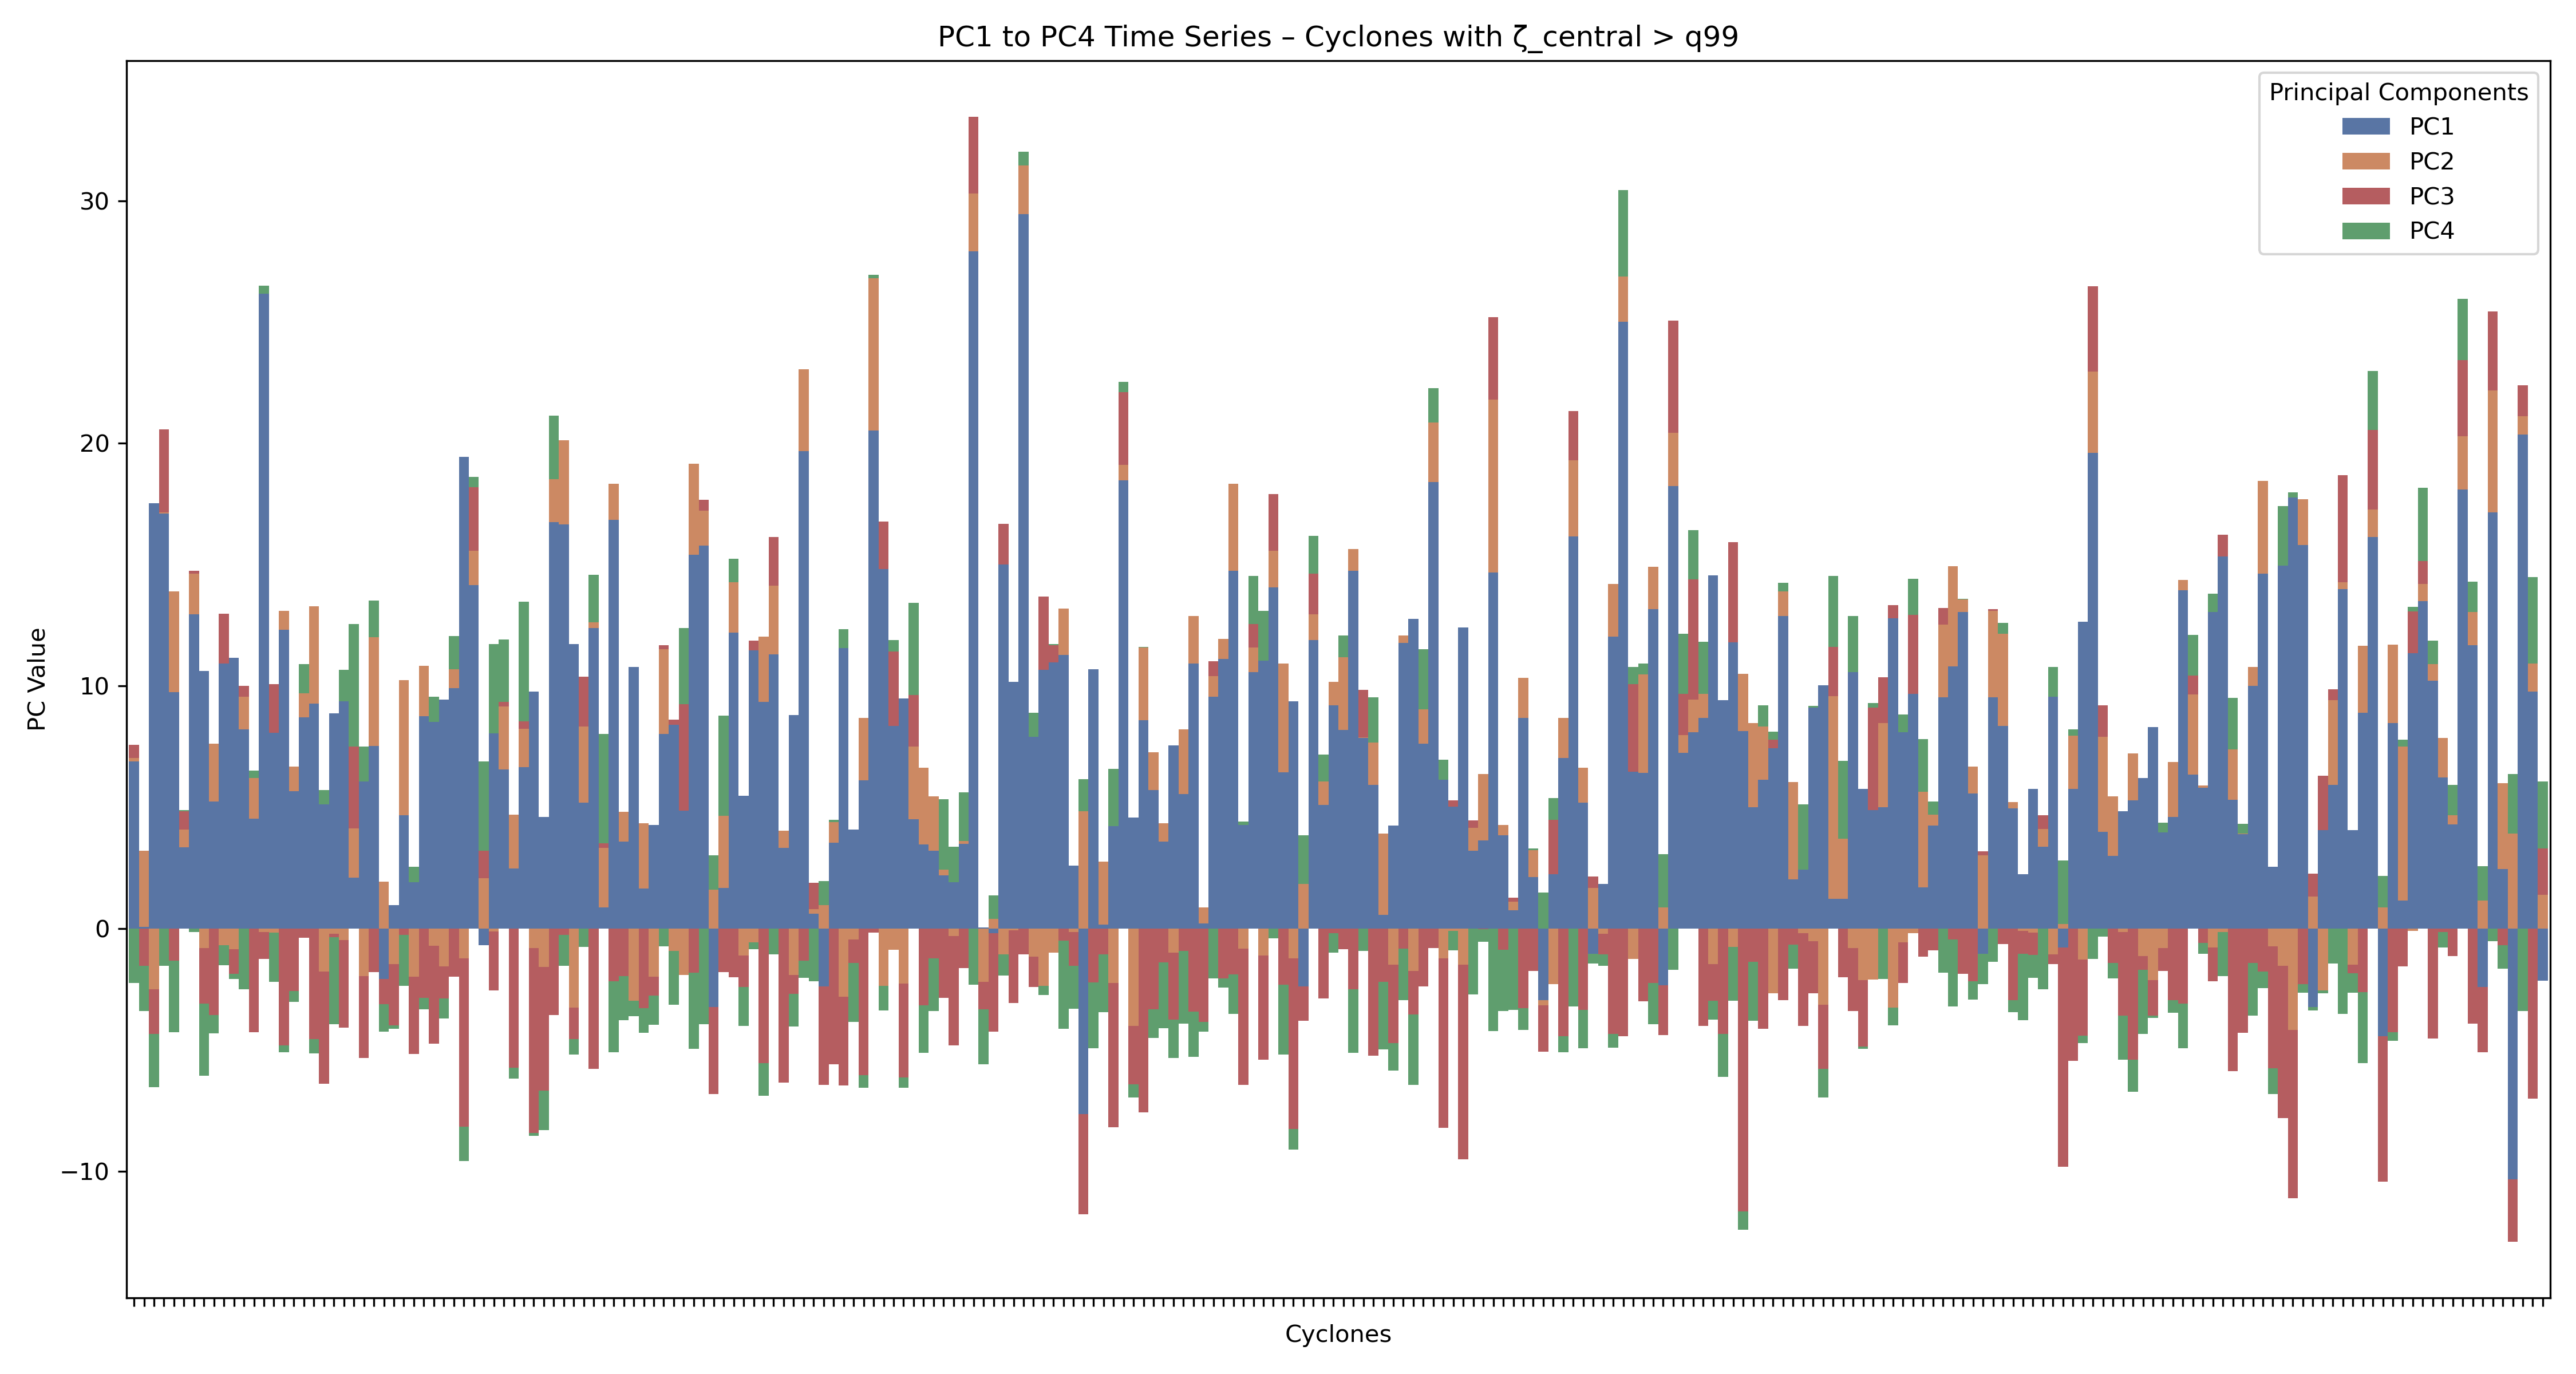
\includegraphics[width=\textwidth]{intense_systems_PCs_stacked_pcs.png}
    \caption{Stacked time series of the first four principal components (PC1–PC4) for each intense
    cyclone (\(\zeta_{850,\mathrm{max}} > q_{99}\)).  
    Positive values are plotted upward and negative values downward, so the coloured bars
    represent the signed contribution of each EOF mode to the energetics of every system.  
    The \(x\)-axis lists the individual cyclones (sorted arbitrarily), while the \(y\)-axis gives the
    PC amplitude (dimensionless).}
    \label{fig:intense_systems_PCs_stacked_pcs}
\end{figure}

\begin{figure}[!htbp]
    \centering
    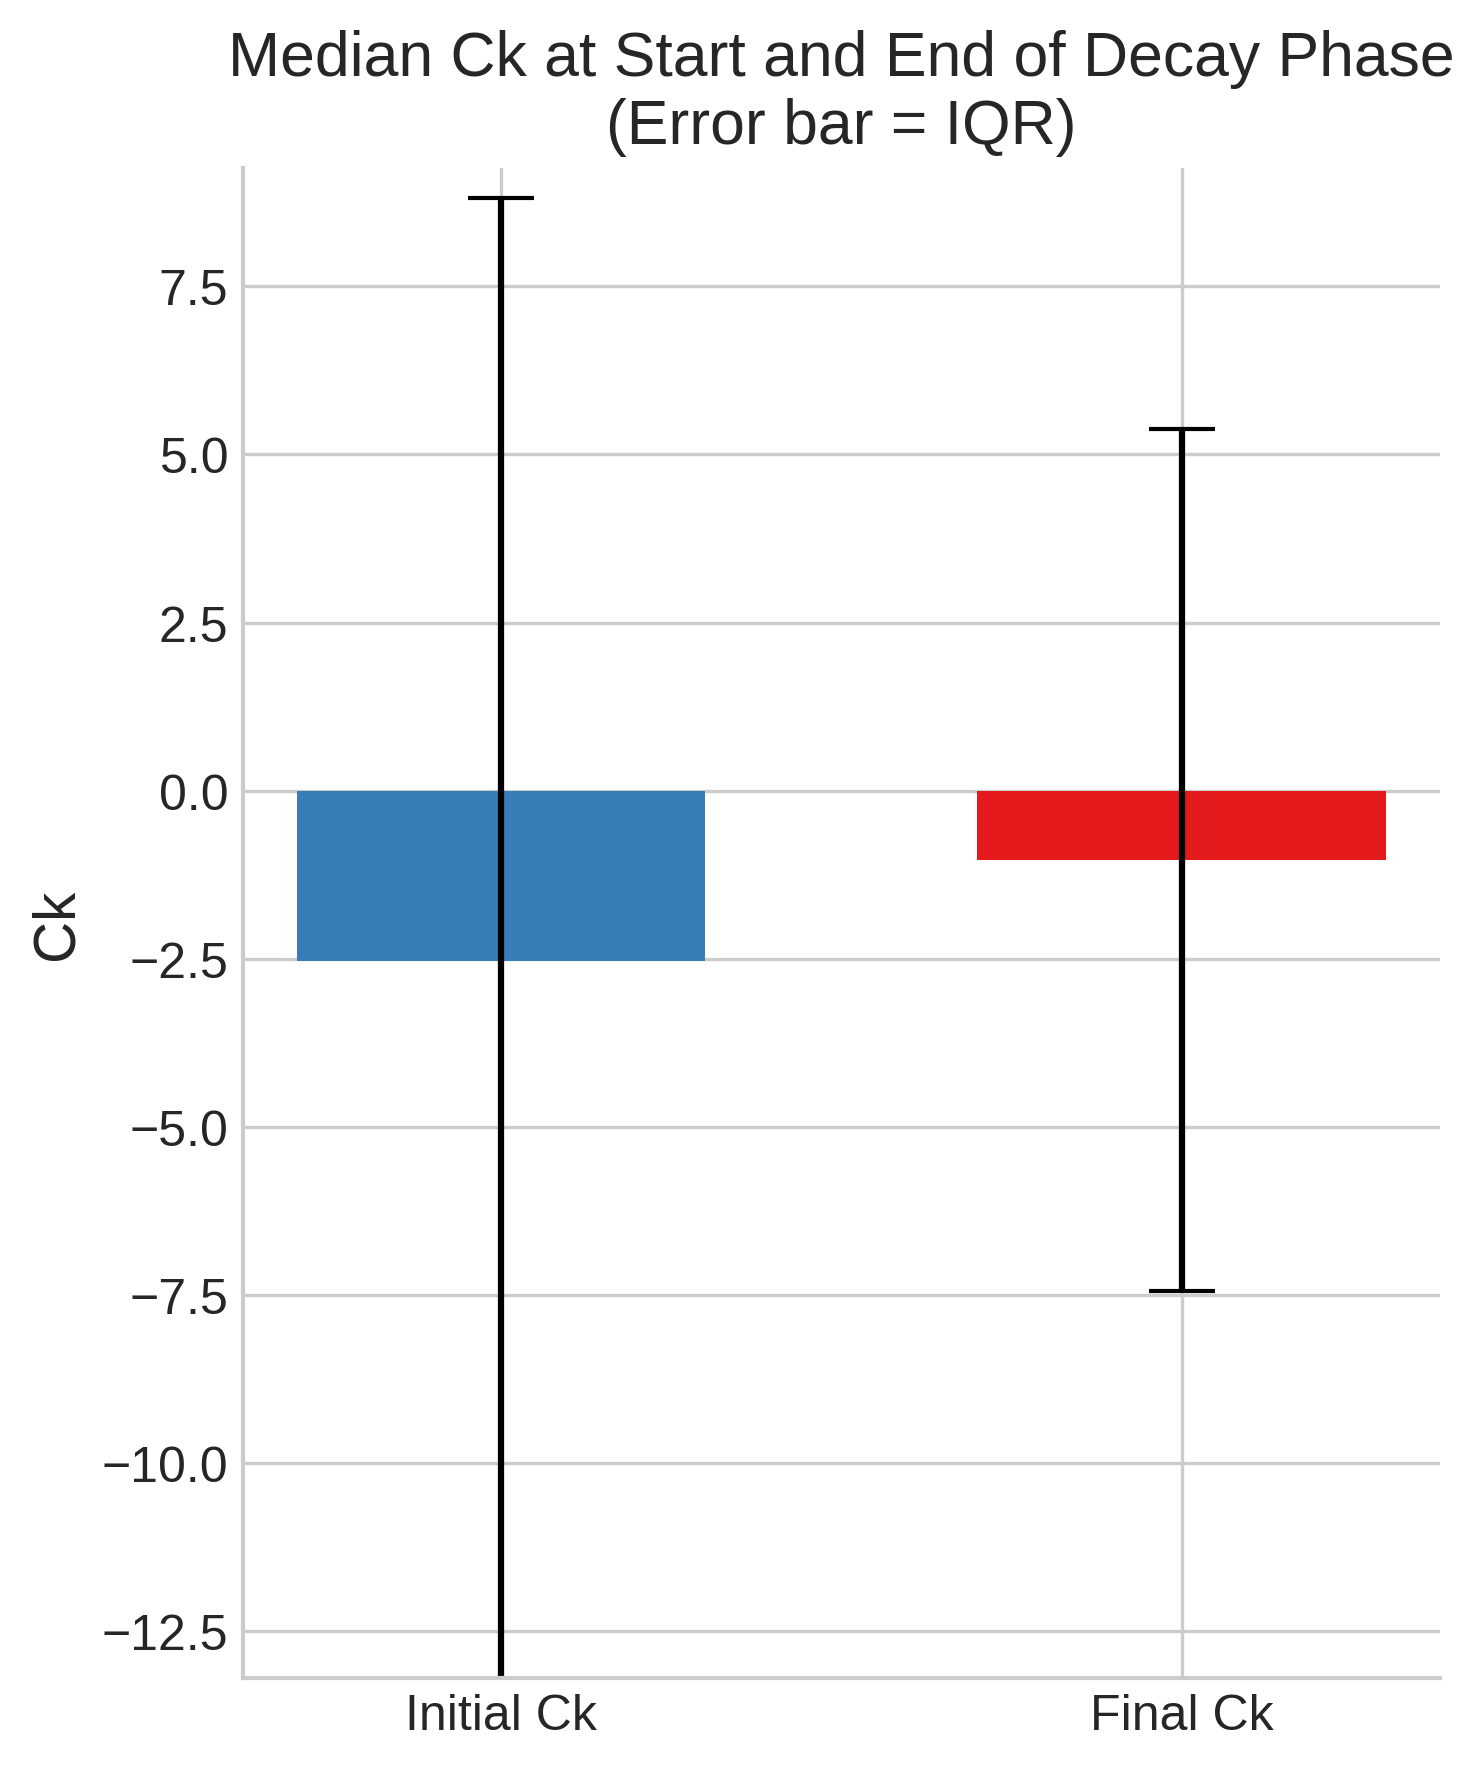
\includegraphics[width=0.55\textwidth]{ck_decay_phase_median_iqr.png}
    \caption{Median barotropic‐conversion term (\(C_k\)) at the start (blue) and end (red) of
    the decay phase, with  the error bars representing the inter-quartile range.}
    \label{fig:ck_decay_phase_median_iqr}
\end{figure}




\end{document}
